\documentclass[11pt]{article}
\usepackage[T1]{fontenc}
\usepackage[utf8]{inputenc}
\usepackage{lmodern}
\usepackage[margin=1in]{geometry}
\usepackage{amsmath,amssymb,amsthm,mathtools}
\usepackage{microtype}
\usepackage[numbers,sort&compress]{natbib}
\usepackage{xcolor}
\usepackage{tikz}
\usetikzlibrary{arrows.meta,positioning}
\usepackage{hyperref}
\hypersetup{pdftitle={The free energy of the spherical random perceptron},pdfauthor={OpenAI},colorlinks=true,linkcolor=blue!50!black,citecolor=blue!50!black,urlcolor=blue!50!black}
\newtheorem{theorem}{Theorem}
\newtheorem{proposition}[theorem]{Proposition}
\newtheorem{lemma}[theorem]{Lemma}
\newcommand{\R}{\mathbb R}
\newcommand{\E}{\mathbb E}
\newcommand{\U}{\mathcal U}
\DeclareMathOperator{\Lip}{Lip}
\allowdisplaybreaks[2]
\setlength{\emergencystretch}{1em}
\title{The free energy of the spherical random perceptron}
\author{OpenAI}
\date{September 24, 2026}
\begin{document}
\maketitle
\begin{abstract}
We prove an exact variational formula for the limiting pressure of the spherical
random perceptron with an arbitrary bounded continuous single-pattern potential.
The formula holds at every fixed positive density and inverse temperature,
with convergence in expectation and in probability.
\end{abstract}

\section{Introduction and statement}
The spherical perceptron is a model of random constraints on a vector of fixed
length. Its partition function measures the spherical volume of configurations
weighted by their responses to independent random patterns. The question here
is whether the pressure has an exact variational description for every fixed
density and temperature, even when the single-pattern reward has no convexity,
concavity, or symmetry.

Let $\alpha,\beta>0$, let $\phi\in C_b(\R;\R)$, and put $M_N=\lfloor\alpha N\rfloor$.
For independent standard Gaussian vectors $g^1,\ldots,g^{M_N}\in\R^N$, define
\[
 S_N=\{x\in\R^N:\|x\|^2=N\},\qquad
 H_N(x)=\sum_{a=1}^{M_N}\phi\left(\frac{g^a\cdot x}{\sqrt N}\right),
 \qquad
 p_N=\frac1N\log\int_{S_N}e^{\beta H_N(x)}\,d\sigma_N(x),
\]
where $\sigma_N$ is the uniform \emph{probability} measure. The sign convention is
positive log-partition pressure; the physical free energy per coordinate is
$-p_N/\beta$.

Write $\U$ for the nondecreasing measurable functions $m:[0,1]\to[0,1]$ and set
\[
 D_m(t)=\int_t^1m(s)\,ds,\qquad
 S(m)=\frac12\int_0^1\left(\frac1{D_m(t)}-\frac1{1-t}\right)dt.
\]
This is a nonnegative extended integral, with $1/0=+\infty$. For $f=\beta\phi$,
let
\[
 V_f(m)=\sup_v\E_B\left[
 f\left(B_1+\int_0^1m(t)v_t\,dt\right)
 -\frac12\int_0^1m(t)v_t^2\,dt\right],
\]
where $B$ is standard Brownian motion with its usual filtration and the supremum
is over progressively measurable real controls of finite expected displayed
cost. This definition applies to bounded continuous $f$ without terminal
smoothness assumptions. In particular, $|V_f(m)|\le\|f\|_\infty$.

\begin{theorem}\label{thm:main}
For every $\alpha,\beta>0$ and every $\phi\in C_b(\R;\R)$,
\[
 \lim_{N\to\infty}\E p_N
 =\inf_{m\in\U}\{\alpha V_{\beta\phi}(m)+S(m)\}
 =:\mathcal P(\alpha,\beta,\phi),
 \qquad
 p_N\xrightarrow{\mathbb P}\mathcal P(\alpha,\beta,\phi).
\]
Trials of infinite entropy have value $+\infty$. No condition that $m=1$ near
$1$ is imposed.
\end{theorem}

The probability normalization of $\sigma_N$ gives the elementary bounds
\[
 \alpha\E f(G)\le\mathcal P(\alpha,\beta,\phi)
       \le\alpha\log\E e^{f(G)},\qquad
 f=\beta\phi,\quad G\sim N(0,1).
\]
At finite $N$, Jensen's inequality inside the spherical integral gives
$\E p_N\ge(M_N/N)\E f(G)$; applying it instead to the outer logarithm
gives $\E p_N\le(M_N/N)\log\E e^{f(G)}$.
For a constant potential $\phi\equiv c$, both bounds coincide at
$\mathcal P=\alpha\beta c$.

\paragraph{The problem and earlier formulas.}
Gardner's storage-volume problem introduced the statistical-mechanical study
of the space of neural-network weights satisfying random constraints
\cite{Gardner1988}. For nonnegative margins, Shcherbina and Tirozzi proved Gardner's
replica-symmetric formula for a truncated logarithm of the feasible spherical
volume below the storage threshold. They also treated a regularization with
Gaussian smoothing and quadratic confinement in a restricted parameter regime
\cite[Theorems~2 and~3]{ShcherbinaTirozzi2003}. These hard-constraint and
regularized observables differ from the arbitrary bounded reward in
Theorem~\ref{thm:main}.

The finite-temperature functional itself has a substantial history.
Gy\"orgyi and Reimann developed the continuous replica-symmetry-breaking
prediction for a spherical perceptron: their equations (3.13), (3.17), and
(3.19)--(3.22) give the terminal evolution and spherical entropy
\cite{GyorgyiReimann2000}. With physical potential $-\phi$ and positive
log-partition pressure, these are the two terms in the formula above.
Montanari and Zhou give a related finite-temperature replica derivation
\cite[Appendix~B]{MontanariZhou2024} in their study of exceptional projections
of Gaussian point clouds. Their rigorous algorithmic theorem concerns
approximate-message-passing values; the replica calculation in that appendix
uses continuation in replica number and limit exchanges. The present theorem
identifies the microscopic quenched pressure using ordinary Gibbs samples.

For an explicit normalization dictionary with \cite{MontanariZhou2024}, set
$h=\phi$, $y=m$, and $\Psi=\beta f_y$ in their equation (100). Their functional
$A$ then satisfies $\alpha\beta A(m,\beta)=\alpha\Psi(0,0)+S(m)$.
Their dimension $d$ and sample count $n$ correspond to $N$ and $M_N$:
pressure per coordinate introduces the factor $n\beta/d\to\alpha\beta$.

\paragraph{Probabilistic methods and spherical entropy.}
The proof builds on the cascade, interpolation, and cavity methods developed
for mean-field spin glasses. Ruelle's Poisson construction gives the hierarchical
weights \cite{Ruelle1987}; Guerra's interpolation supplies the classical
replica-symmetry-breaking comparison \cite{Guerra2003}; and the extended
variational principle of Aizenman, Sims, and Starr places fixed-size cavity
increments at the center of the pressure calculation \cite{AizenmanSimsStarr2003}.
The spherical entropy is related to the Crisanti--Sommers functional
\cite{CrisantiSommers1992} and its rigorous formulation by Talagrand
\cite[Equation~(1.11)]{Talagrand2006Spherical}. These Gaussian spin-glass
results provide methods and comparison formulas; the nonlinear pattern
Hamiltonian requires the arguments given below.

\paragraph{The obstacle and the main ideas.}
Although the patterns are Gaussian, their nonlinear sum $H_N(x)$ is generally
not a Gaussian process in $x$. A Gaussian mixed-spin pressure formula therefore
does not directly give Theorem~\ref{thm:main}. Nor does an arbitrary $\phi$
provide a convexity sign for a usual comparison interpolation. The proof uses
two different kinds of increments: adding a random pattern, and adding spin
coordinates.

\begin{figure}[t]
\centering
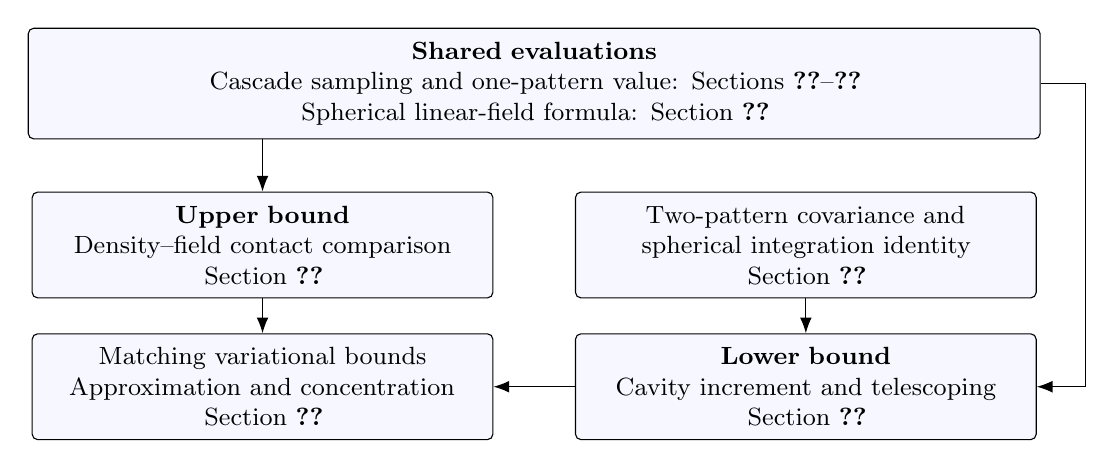
\begin{tikzpicture}[
 box/.style={draw,rounded corners=2pt,align=center,text width=5.5cm,
 minimum height=1.05cm,font=\small,fill=blue!3,inner sep=5pt},
 >={Latex[length=2mm]}]
\node[box,text width=12.5cm] (shared) at (0,0)
 {\textbf{Shared evaluations}\\
 Cascade sampling and one-pattern value: Sections~\ref{sec:prelim}--\ref{sec:value}\\
 Spherical linear-field formula: Section~\ref{sec:spherical}};
\node[box] (upper) at (-3.45,-2.05)
 {\textbf{Upper bound}\\
 Density--field contact comparison\\Section~\ref{sec:upper}};
\node[box] (bulk) at (3.45,-2.05)
 {Two-pattern covariance and\\spherical integration identity\\Section~\ref{sec:bulk}};
\node[box] (finish) at (-3.45,-3.85)
 {Matching variational bounds\\Approximation and concentration\\Section~\ref{sec:completion}};
\node[box] (cavity) at (3.45,-3.85)
 {\textbf{Lower bound}\\
 Cavity increment and telescoping\\Section~\ref{sec:cavity}};
\draw[->] (shared.south -| upper.north)--(upper.north);
\draw[->] (shared.east)--(7.0,0)--(7.0,-3.85)--(cavity.east);
\draw[->] (bulk)--(cavity);
\draw[->] (upper)--(finish);
\draw[->] (cavity)--(finish);
\end{tikzpicture}

\caption{The two bounds share the cascade one-pattern value and the spherical
linear-field calculation. The upper argument uses a contact comparison; the
lower argument identifies the covariance generated by added coordinates.
Arrows indicate the main proof inputs; they do not specify exchanges of limits.}
\label{fig:proof}
\end{figure}

The overlap $R(x,x')=x\cdot x'/N$ measures the agreement of two Gibbs samples.
Small Gaussian perturbations impose the Ghirlanda--Guerra identities on its
limiting array. The Dovbysh--Sudakov representation and Panchenko's support
and ultrametricity theorems then describe that array by an ordered overlap law
\cite{Panchenko2010DovbyshSudakov,Panchenko2010Support,Panchenko2013Ultrametricity}.
Finite Ruelle cascades evaluate functions of this law. We prove the sampling
and marked transformations needed here, with credit to the joint marked-law
calculus of Panchenko and Talagrand \cite{PanchenkoTalagrand2007Cascades}.
The independent Gaussian remainder on each replica visit is retained even
when two visits select the same leaf.

The upper bound adapts Mourrat's Hamilton--Jacobi approach to nonconvex
spin glasses. Enrichment by a cascade Gaussian field is used in the work of
Mourrat and Panchenko \cite[Equation~(1.6) and Theorem~1.1]{MourratPanchenko2020}.
The comparison here follows Mourrat's contact-point supersolution argument
\cite[Section~4, proof of Theorem~4.1]{Mourrat2021Nonconvex}; its vector-spin
extension appears in \cite[Theorem~3.4 and Section~5]{Mourrat2023VectorUpper}.
In this argument, perturbation parameters are selected at a contact minimum,
where curvature and concentration enforce joint overlap identities. These
identities order the spin and label overlaps. We use Panchenko's
synchronization argument \cite[Section~4, Lemma~2]{Panchenko2015Multispecies}
in the monotone-coupling formulation of Mourrat
\cite[Proposition~5.2 and Theorem~5.3]{Mourrat2021Nonconvex}.
The cited pressure bounds concern Gaussian Hamiltonians. For the nonlinear
pattern Hamiltonian, we use Poissonized density as the time variable and
the tail-order property of the one-pattern value to obtain the comparison.

For the lower bound, remove two patterns and restore them as independent
marks. Their first and second moments show that the covariance of the field
acting on new coordinates is a deterministic function of the spin overlap.
Tangential integration on the sphere identifies that function with the
derivative of spherical entropy. The ensuing cavity increment is therefore
bounded below by the same variational functional. A uniform spherical-field
calculation allows the cavity size to tend to infinity after the bulk limit.
Identifying the cavity parameters through overlap observables is related to
the critical-point approach of Chen and Mourrat
\cite[Sections~6--7]{ChenMourrat2025Critical}. Their results concern Gaussian
vector-spin models and do not directly apply here; the two-pattern removal
and spherical integration identity provide the relations needed in this model.
Figure~\ref{fig:proof} shows where the two bounds share inputs.

\paragraph{Proof structure.}
Sections~\ref{sec:prelim} and~\ref{sec:value} develop the cascade calculus and
an order property of the one-pattern value. Section~\ref{sec:spherical}
evaluates the spherical linear-field term, including the uniformity required
in the cavity limit. Section~\ref{sec:upper} proves the upper bound by an
affine comparison for negative pressure. For the lower bound,
Section~\ref{sec:bulk} uses two-pattern removal to identify bulk gradient
covariances and a spherical integration identity to determine them explicitly.
Section~\ref{sec:cavity} evaluates and telescopes cavity increments.
Section~\ref{sec:completion} passes from smooth potentials to bounded
continuous ones and proves concentration.



\section{Quantiles and cascade preliminaries}\label{sec:prelim}

The upper comparison and the cavity argument both evaluate the effect of a fresh Gaussian pattern on a limiting Gibbs measure. We first encode its overlap law by a quantile and a finite cascade. The marked-cascade calculation then specifies exactly what is shared by replicas and what must be sampled afresh at each visit.

Throughout the proof, $f=\beta\phi$. Sections~\ref{sec:prelim}--\ref{sec:cavity} assume $f\in C_c^\infty(\mathbb R)$; Section~\ref{sec:completion} removes this assumption. All perturbations and enrichments of the model in the proof will have their own auxiliary randomness, independent of the patterns unless stated otherwise. Expected log-partition functions for those models include expectation in this randomness (with parameter values held fixed, unless a further averaging in parameters is specified).

Up to changes irrelevant to the functionals, a trial $m$ is the cumulative distribution function, restricted to $[0,1)$, of a probability $\mu$ on $[0,1]$ (put any remaining mass at 1). Let $q$ be a nondecreasing quantile function, viewed modulo null sets on $(0,1)$. We will use $V(q)$ and $S(q)$ for the value and entropy defined above in this parametrization; $D_q=D_m$. In particular

\begin{equation*}
D_q(t)=1-t-\int_0^1(q(u)-t)_+\,du.
\end{equation*}

In scalar products of functions of the quantile parameter $u$, the integration is on $(0,1)$ with Lebesgue measure.

Here is some notation for finite quantiles. Use $k\ge1$ consecutive intervals of lengths $w_i>0$, $0\le i\le k-1$, of sum 1. Write $\zeta_i=\sum_{j<i}w_j$, including $\zeta_0=0,\ \zeta_k=1$. A step $q$ has values $0\le q_0\le\cdots\le q_{k-1}\le1$; set $q_{-1}=0, q_k=1$. Another kind of nonnegative nondecreasing function we will use, with no bound by 1 required, is $h$ describing field parameters; similarly write $h_i$ for step values on such intervals.

We use actual Gibbs samples (replicas), i.i.d. given the Gibbs measure, without any continuation in replica number; $\langle\ \rangle$ denotes Gibbs expectation, including for arbitrarily many such samples. The spin overlap on $S_N$ is $R(x,x')=x\cdot x'/N$, giving an array $R_{\ell j}$. In enriched models replicas include extra labels.

\subsection{Overlap identities and finite cascades}

For the intervals above, use a Ruelle probability cascade (RPC) \cite[Section~3]{Ruelle1987} of depth $k-1$ with parameters $\zeta_1,\ldots,\zeta_{k-1}$. Its leaf weights $v_\gamma$, summing to 1, are obtained by normalizing the products of Poisson weights along paths: for edges from each vertex at level $i-1$ to its children at level $i$ use an independent Poisson process on $(0,\infty)$ of intensity $\zeta_i x^{-1-\zeta_i}dx$, whose points can be arranged in decreasing order. At depth zero there is just weight 1. For two leaves the common level is the depth $\gamma\wedge\eta$ of their last common vertex, including $k-1$ if equal.

We use the standard overlap-array theory developed in \cite{Panchenko2013Book,Panchenko2013Ultrametricity}. The deep input is Panchenko's ultrametricity theorem \cite[Theorem~1]{Panchenko2013Ultrametricity}. We state precisely the other facts needed and explain their use below. The Ghirlanda--Guerra (GG) law \cite{GhirlandaGuerra1998} for an array $B$ with constant diagonal says that, given entries among the first $n$ replicas, $n\ge2$, the conditional law of $B_{1,n+1}$ is

\begin{equation*}
\frac1n\,\mathcal L(B_{12})+\frac1n\sum_{2\le j\le n}\delta_{B_{1j}}.
\end{equation*}

This is an identity for the law that includes disorder averaging. We use Panchenko's ultrametricity theorem: a weakly exchangeable random Gram array (symmetric positive semidefinite in finite restrictions, bounded here, with fixed diagonal normalized or rescalable to 1) satisfying the GG identities has ultrametric off-diagonal overlaps, $B_{23}\ge\min(B_{12},B_{13})$ a.s. For precision, the Dovbysh--Sudakov representation
\cite[Proposition~1]{Panchenko2010DovbyshSudakov} represents a normalized
Gram array as $h^\ell\cdot h^j+a_\ell\mathbf1_{\{\ell=j\}}$, with
$a_\ell\ge0$ and a directing measure on the Hilbert unit ball.
The support theorem \cite[Theorem~2(a)]{Panchenko2010Support}, applied to
the off-diagonal GG identities, makes $\|h^\ell\|^2$ equal to the
supremum of the off-diagonal support almost surely. The represented
inner-product array thus has deterministic diagonal; the off-diagonal
identities give its full GG identities, to which the ultrametricity theorem
applies. This verifies the Gram-array formulation without identifying the
original diagonal with the directing-vector norm. Here one can take entries off the diagonal nonnegative for this theorem: nonnegativity itself follows under the GG law in these assumptions. Indeed if an event $B_{12}<-\delta$ with $\delta>0$ has mass $b>0$, the all-pairs off-diagonal event of this kind among $n$ replicas can be extended to $n+1$ with conditional probability at least $b$ on this event, by exchangeability, the GG law and a union bound. This for arbitrarily large $n$ contradicts positivity of the quadratic form on the all-ones vector.

We also use the standard finite RPC overlap result: for replicas sampled from its weights (and averaging the cascade randomness), their off-diagonal common-level array has two-replica level probabilities $w_i$ and satisfies the GG identities. In particular a scalar array with values in $[0,1]$ and diagonal 1 satisfying the Gram, exchangeability and GG assumptions above can be evaluated by finite cascades after rounding its off-diagonal overlaps by a nondecreasing finite-valued map into $[0,1]$. The law of the rounded array off the diagonal is the one with overlaps given by values at the RPC levels, using the ascending list of values of positive probability and their probabilities. Indeed the rounded array is still ultrametric and satisfies GG. These properties determine its law with the given two-replica probabilities: given the first $n$, at each overlap threshold in the list, for each existing equivalence class at that threshold the chance the next replica belongs to it is specified by the GG formula using a representative. (Equivalence here means equal indices or overlap at least the threshold.) The nested classes and all these conditional probabilities determine the probabilities of all possible joining locations, hence of the new overlaps. This gives uniqueness starting with the two-replica law.

\paragraph{The finite-cascade sampling law.}
The complete weights-and-ancestry law was identified by Bolthausen and
Sznitman \cite[Theorem~2.2 and Proposition~1.4]{BolthausenSznitman1998}.
Here is a direct verification of the RPC law just used, including the
conditioning on the whole sampled tree. Write $D=k-1$ and $z_i=\zeta_i$,
so $0=z_0<z_1<\cdots<z_D<z_{D+1}=1$.
At a vertex whose outgoing Poisson exponent is $b$, absorb each independent
descendant total $T(C)$ into its edge weight: $y=uT(C)$. The marked intensity
becomes
\[
 b y^{-1-b}\,dy\;T(C)^b\,\mathbb P(dC).
\]
The descendant subtrees therefore have independent laws biased by their
totals to power $b$, independently of the new edge masses. An incoming
bias by the parent total to power $a$, where $0\le a<b$, depends only on
the sum of those masses and preserves this independence. The required
moments are finite because the next Poisson exponent is strictly larger;
at leaves the descendant total is one.

For stable Poisson jumps of exponent $b$, let $S$ be their sum and bias
their law by $S^a/\E S^a$. The probability of a specified partition of
$n\ge1$ visits into $j$ nonempty blocks of sizes $n_1,\ldots,n_j$ is
\[
 \frac{\Gamma(1-a)}{\Gamma(n-a)}
 \prod_{\ell=1}^{j-1}(\ell b-a)
 \prod_{r=1}^{j}\frac{\Gamma(n_r-b)}{\Gamma(1-b)}.
\]
To obtain the formula, insert
$S^{a-n}=\Gamma(n-a)^{-1}\int_0^\infty t^{n-a-1}e^{-tS}\,dt$
in the sum over distinct sampled Poisson points, use the Poisson factorial
moment identity, and then integrate with the stable Laplace transform
$\E e^{-tS}=e^{-ct^b}$. All terms are nonnegative, so these integrations
are justified by monotone convergence. Ratios of the displayed probabilities
give $(n_r-b)/(n-a)$ for joining an occupied child and $(jb-a)/(n-a)$
for taking a new child; the first visit is assigned to a new child.

Iterating the independent subtree decomposition gives these local split
laws with $(a,b)=(z_{i-1},z_i)$. The likelihood of a sampled nested
partition factors over its occupied vertices. Conditional on the visits to a
child, observations below that child concern its independent subtree; they
therefore give no further information about the parent's normalized masses.
Thus the same local ratios hold given the entire sampled partition. If
$C_0\supset C_1\supset\cdots\supset C_i=C$ is the path to an occupied
depth-$i$ class, with $n_{C_0}=n$, its next-visit probability is
\[
 \prod_{j=1}^i\frac{n_{C_j}-z_j}{n_{C_{j-1}}-z_{j-1}}
 =\frac{n_C-z_i}{n}.
\]
With one existing replica this probability is $1-z_i$; differences give
the pair-level probabilities $w_i$. For a class containing replica 1,
the displayed ratio is exactly the GG mixture for its threshold indicator.
These indicators span all functions of the finite common level, proving GG
with arbitrary tests of the previously sampled tree. The conditioning is on
the nested partition of replica indices, not on numerical Poisson ranks or
realized marks. Depth zero is deterministic; the endpoint exponents zero
and one do not create Poisson branching levels.

\subsection{Marked cascade transformations}

We next describe what happens to both weights and marks when a cascade is
reweighted. The joint law is needed when two removed patterns are restored:
invariance of the weights alone would not identify products of their
observables. The marked Poisson calculation is developed in
\cite[Lemmas~2.1 and~3.1, Corollary~3.2]{PanchenkoTalagrand2007Cascades};
we give the conditional version needed here.

Marks may include common root data, independent of all Poisson weights.
Given ancestor marks, children receive independent marks according to a
probability kernel, also independently of the Poisson weights. For example, a Gaussian field with nonnegative
nondecreasing covariance levels $b_i$ has independent vertex increments of
variances $b_0$ at the root and $b_i-b_{i-1}$ at depth $i\ge1$.
Let $X_{k-1}$ be a leaf log factor depending on the marked path and define
backward, at each vertex,
\begin{equation}\label{eq:marked-recursion}
 X_{i-1}=\zeta_i^{-1}\log E_i e^{\zeta_i X_i},
 \qquad i=k-1,\ldots,1,
\end{equation}
where $E_i$ integrates the child mark given the path through depth $i-1$.
We assume these recursions are finite, with integrable root value whenever
an unconditional expectation is taken.

\begin{lemma}[Marked cascade law]\label{lem:marked-cascade}
In the preceding setting, put
$L_X=\log\sum_\gamma v_\gamma e^{X_{k-1}(\gamma)}$.
The following conclusions hold.
\begin{enumerate}
\item Conditional on root data,
\[
 E[L_X\mid\text{root}]=X_0,\qquad
 E[(L_X-X_0)^2\mid\text{root}]\le C_\zeta,
\]
where $C_\zeta$ depends only on the fixed cascade parameters.
\item After multiplication by $e^{X_{k-1}}$ and normalization, the weights,
up to tree relabeling, again have the ordinary cascade law. Jointly with
these weights, the child mark kernels are tilted by
$e^{\zeta_i(X_i-X_{i-1})}$. The transformed unmarked tree is independent
of root data. Given a finite sampled tree shape, the root has its original
law and the marks are generated by these tilted kernels, independently
for distinct children conditional on their ancestors.
\item Suppose the marks consist of independent components: their root
variables are independent, their child kernels factor over components
with each kernel depending only on its own ancestral component marks,
and $X_{k-1}$ is a sum of functions of the separate component paths.
Then the recursions are additive and the tilted kernels factor. In
particular the components remain independent conditional on a sampled
finite tree shape.
\end{enumerate}
\end{lemma}

\begin{proof}
Multiply each level-$i$ edge weight by $e^{X_i-X_{i-1}}$ and reorder the
children. The conditional fractional moment
\[
 E_i e^{\zeta_i(X_i-X_{i-1})}=1
\]
shows that Poisson mapping preserves the edge intensity and tilts its mark
kernel by precisely this factor. Only this fractional moment is required;
see also \cite[Appendix, Proposition~A.2]{BolthausenSznitman1998}.
A first moment of $e^{X_{k-1}}$ is unnecessary, a distinction that will
matter for the canonical quadratic factors in Section~\ref{sec:spherical}.

The mapping is applied from the leaves upward. Its induction preserves the
ordinary law of the entire transformed unmarked subtree, independently of
ancestor marks. Indeed, at a parent regard the child mark together with its
already transformed unmarked descendant subtree as one mark. By induction
the latter has a fixed law independent of the path. The parent multiplier
depends only on the path and child mark, so mapping gives the ordinary edge
intensity times the tilted child kernel times the unchanged descendant
law. The unit fractional moment removes any scale depending on ancestors.
This proves the joint-law assertion. Sampling labels depends only on the
unmarked tree; conditioning on their shape therefore leaves the root law
and the stated mark kernels intact. For independent components, the
exponential moments in \eqref{eq:marked-recursion} factor at each step,
proving the last assertion. Independence of the root components is part
of this hypothesis; conditional independence given shared random root
data alone would not suffice after averaging those data.

For the first assertion, let $T$ and $T'$ be the original and transformed
sums of unnormalized leaf products. The product of edge multipliers along
a path is $e^{X_{k-1}-X_0}$, hence
\[
 L_X=X_0+\log T'-\log T.
\]
Conditional on the root, both totals have the ordinary cascade total's
law. That total is positive and finite and has finite log second moment.
To see this, sum descendant totals one level at a time: a Poisson sum
of exponent $\zeta_i$ with independent positive factors of finite
$\zeta_i$-moment is positive stable of index $\zeta_i$, up to scale.
Successive exponents increase, so the necessary moments exist. A positive
stable variable has positive moments of every smaller order and finite
negative moments, the latter also following from its Laplace transform.
These imply the claimed log moment. The two conditional marginal laws
therefore give zero mean and a fixed second-moment bound for
$\log T'-\log T$; independence of the totals is not needed.
At depth zero $L_X=X_0$ and no Poisson calculation is required.
\end{proof}

There is one further distinction when Gaussian marks represent replica
arrays. Suppose the shared field $Z(\gamma)$ has covariance levels $b_i$
and the desired diagonal variance is $d\ge b_{k-1}$. Its evaluations on
replica visits are
\begin{equation}\label{eq:replica-residual}
 G^\ell=Z(\gamma^\ell)+\sqrt{d-b_{k-1}}\,\eta_\ell,
 \qquad (\eta_\ell)_{\ell\ge1}\text{ independent standard Gaussians}.
\end{equation}
The residuals are independent of the shared field and labels, and remain
independent even when two visits choose the same leaf.
Thus distinct replicas then have covariance $b_{k-1}$, while each has
variance $d$. For a leaf factor, integrate the residual before applying
\eqref{eq:marked-recursion}. After reweighting, an observable on a visit
uses the ordinary tilt of that residual's law, separately for each visit.
More generally the same rule applies to any fresh terminal marks averaged
inside a leaf factor.

\subsection{Passing fresh fields through overlap limits}

The following passage explains why finite cascades evaluate the fresh
patterns and cavity fields of a limiting overlap array. Here the base
Gibbs measure may depend on disorder, and a fresh Gaussian field may have
a covariance determined by that base disorder.

\begin{lemma}[Bounded fresh-field passage]\label{lem:fresh-field-passage}
Suppose that the covariance arrays of finitely many conditionally centered Gaussian
fresh fields, together with the needed bounded base observables, are
uniformly bounded and converge in law on every finite set of base
replicas. Conditional on base data and replicas, the fields have the
specified joint Gaussian law; different components are conditionally
independent when so specified. Let $W$ be a bounded continuous function
of the fresh marks and base observables of one replica, with fixed bounds
$0<a\le W\le b<\infty$. Then both the expected log integral
$E\log\langle W\rangle$ and bounded continuous tests of the fresh
evaluations and converging base observables under reweighting by $W$
pass to limits determined by those finite array laws. The same
holds after adjoining an independently integrated trial spin with a fixed
compactly supported law.
\end{lemma}

\begin{proof}
For a bounded continuous test $\Psi$ of $n$ replicas, the reweighted
expectation is
\begin{equation}\label{eq:bounded-replica-quotient}
 E\left[
 \frac{\left\langle\Psi\prod_{\ell=1}^nW(x^\ell)\right\rangle}
      {\langle W\rangle^n}\right].
\end{equation}
Approximate $s^{-n}$ and $\log s$ uniformly by polynomials on $[a,b]$.
Each resulting term is an expectation on finitely many base replicas,
with the additional replicas evaluating the same fresh fields. Such
terms converge because finite-dimensional Gaussian expectations are
continuous in the covariance matrix, including degenerate matrices.
The uniform approximation error then proves both assertions. Extra
trial-spin integration can be included in the reference probability
measure and in the same calculation.
\end{proof}

For the pattern and cavity fields below, the limiting off-diagonal
covariances are continuous nonnegative nondecreasing functions of a
scalar ultrametric GG overlap, bounded by their respective diagonal
variances. Round that overlap down by nondecreasing finite-valued maps with
error tending uniformly to zero, retaining the true field diagonals.
The rounded overlap law and these ordered covariance levels have the
finite-cascade representation above. If a fresh
field's diagonal exceeds its top off-diagonal covariance, use
\eqref{eq:replica-residual} in each polynomial term. Its independent
residuals are thereby averaged at the leaf before the marked recursion.
This is forced by the finite-replica covariance matrix, rather than a
choice of a shared leaf mark. As the rounded covariances approach their
original values, Gaussian continuity and the uniform polynomial error
give the desired limit. Section~\ref{sec:cavity} supplies a separate
truncation estimate for its unbounded spherical factor.

\subsection{Gaussian differentiation at fixed size}\label{sec:gaussian-calculus}

We will also differentiate partition integrals at fixed dimension, before
taking overlap limits. Let $\rho$ be a reference probability measure,
possibly random, independent of the added Gaussian fields conditional on
its base data. For centered Gaussian energy $G_s$ whose bounded covariance
$K_s$ varies affinely with $s$, Gaussian integration by parts gives
\begin{equation}\label{eq:gaussian-covariance-derivative}
 \frac{d}{ds}E\log\int e^{G_s(x)}\,d\rho(x)
 =\frac12 E\left\langle
       \dot K_s(x^1,x^1)-\dot K_s(x^1,x^2)\right\rangle_s.
\end{equation}
Explicit deterministic shifts are differentiated separately. This formula,
its integral along the covariance segment, and its one-sided endpoint
versions apply to the bounded-spin, finite-cascade integrals used below.
Ordinary coupling derivatives, including Gaussian insertions and products
of Gibbs averages with bounded continuous overlap tests, may likewise
be passed through expectation.

Here are moment bounds justifying these uses despite the infinitely many
cascade leaves. For $r\ge1$, Jensen bounds positive powers of a Gaussian
exponential integral by the integral of $e^{rG}$. For any $r>0$ it also gives
\[
 \left(\int e^G\,d\rho\right)^{-r}
 \le \exp\left(-r\int G\,d\rho\right)
 \le \int e^{-rG}\,d\rho.
\]
Uniform covariance bounds and Gaussian exponential moments therefore
control positive and inverse moments, also with polynomial Gaussian
insertions by H\"older's inequality. Bounded pattern energies independent
of the added fields may be absorbed into $\rho$ after normalization;
their normalization has the needed moments also for a Poisson number of
patterns. These estimates hold locally uniformly in bounded coupling
parameters at each fixed dimension.

To justify \eqref{eq:gaussian-covariance-derivative} directly, first replace
$\rho$ by its empirical measure from independent samples conditional on
$\rho$, also independent of the fresh Gaussian fields. For the spheres
and countable leaf coordinates in this paper, the state space is
separable and the fields are continuous in the spin coordinate at each
leaf. Conditional laws of large numbers give convergence of the weighted
integrals and their continuous replica tests; polynomial insertions can
first be truncated. The moment bounds pass these statements through
expectation. Couple the fields on a segment as
$\sqrt{1-s}G_0+\sqrt{s}G_1$. Exponentials involving
$|G_0|+|G_1|$, with polynomial factors when needed, give uniform moment
bounds, and the bounded covariance terms on the right side of
\eqref{eq:gaussian-covariance-derivative} are continuous in $s$.
The integral identity thus passes from empirical measures by bounded
convergence in $s$, including one-sided derivatives at the endpoints.
The same local bounds give ordinary coupling differentiation and uniform
integrability. The canonical integral with unbounded spins in
Section~\ref{sec:spherical} is instead treated by its explicit recursion.

\section{The single-pattern value and its order property}\label{sec:value}

Adding one independent pattern changes the log partition function by an expected log Gibbs integral. We first identify that integral with the control value $V(q)$, then prove the tail-integral order that supplies the sign in the upper comparison. Throughout this section $f\in C_c^\infty(\R)$, as stipulated in Section~\ref{sec:prelim}.

\paragraph{The cascade integral and control representation.}
Fix a finite quantile with the notation $q_i,w_i,\zeta_i$ of Section~\ref{sec:prelim}. On its cascade let $z(\gamma)$ be a centered Gaussian mark with covariance $q_{\gamma\wedge\eta}$, independent of the cascade weights. We claim that
\begin{equation*}
 V(q)=\E\log\sum_\gamma v_\gamma\,
       \E_G\exp f\bigl(z(\gamma)+\sqrt{1-q_{k-1}}\,G\bigr),
 \qquad G\sim N(0,1).
\end{equation*}
Here the outer expectation includes the cascade and all its shared Gaussian marks. The inner expectation averages the residual noise of one replica visit. Different visits use independent copies of $G$, even if their labels coincide. Thus the shared field has covariance $q_{\gamma\wedge\eta}$ between distinct replicas, while every replica's total field has variance one.

For $s\ge0$ and $d\ge0$, write
\[
 \mathcal T_{s,d}g(x)=
 \begin{cases}
 d^{-1}\log\E\exp\bigl(dg(x+\sqrt{s}\,G)\bigr),&d>0,\\
 \E g(x+\sqrt{s}\,G),&d=0.
 \end{cases}
\]
The operator $\mathcal T_{0,d}$ is the identity, so zero-length intervals require no separate convention. Starting with $U_k=f$, define backward functions by
\[
 U_{i-1}=\mathcal T_{q_i-q_{i-1},\zeta_i}U_i,
 \qquad i=k,k-1,\ldots,0.
\]
Recall that $q_{-1}=0$, $q_k=1$, $\zeta_0=0$, and $\zeta_k=1$. The first backward step, from $1$ to $q_{k-1}$, is the logarithm of the residual average in the displayed cascade integral. The marked-cascade recursion handles levels $k-1$ through $1$, and the final ordinary expectation averages the root mark of variance $q_0$. Consequently that integral equals $U_{-1}(0)$.

To identify this number with the control value, interpolate the recursion on each interval $[q_{i-1},q_i]$ by
\[
 U(t,x)=\mathcal T_{q_i-t,\zeta_i}U_i(x).
\]
These pieces agree at their endpoints and solve the backward equation
\[
 \partial_tU+\frac12\partial_{xx}U
       +\frac{m(t)}2(\partial_xU)^2=0,
 \qquad U(1,x)=f(x),
\]
where $m(t)=\zeta_i$ in the interior of that interval. The heat semigroup and exponential transform give this equation directly. Differentiating the Gaussian formulas shows that the first and second spatial derivatives are bounded, including their limits at interval endpoints, for the fixed finite recursion.

For an admissible control $v$, set
\[
 X_t^v=B_t+\int_0^t m(s)v_s\,ds.
\]
It\^o's formula on successive intervals and completion of the square give
\[
 \E\left[f(X_1^v)-\frac12\int_0^1m(t)v_t^2\,dt\right]
 =U_{-1}(0)-\frac12\E\int_0^1m(t)
       \bigl(v_t-\partial_xU(t,X_t^v)\bigr)^2\,dt.
\]
Bounded derivatives and the finite expected control cost justify the expectations, or one may first localize. This proves the upper bound by $U_{-1}(0)$ for every control. Equality is attained with $v_t=\partial_xU(t,X_t^v)$: this feedback is bounded and Lipschitz in space, so its stochastic equation has an adapted solution of finite cost. Hence $V(q)=U_{-1}(0)$, proving the claimed cascade identity. Brownian variational formulas \cite[Theorem~3.1]{BoueDupuis1998} and the control formulation of the Parisi PDE \cite[Theorem~3]{AuffingerChen2015} provide the background for this representation; the calculation above verifies it for the arbitrary smooth terminal function needed here.

\paragraph{Continuity and general overlap laws.}
For a Lipschitz terminal function with $L=\Lip(f)$, the control supremum can be restricted to $|v|\le L$. Indeed clipping $v$ to this interval changes the terminal reward by at most $L\int m|v-\operatorname{clip}(v)|$, while the saved quadratic cost is at least this quantity. Comparing the same clipped controls for $m$ and $m'$ therefore gives
\[
 |V_f(m)-V_f(m')|\le\frac32 L^2\|m-m'\|_1.
\]
Area integration between distribution functions and their quantiles gives
$\|m-m'\|_1=\|q-q'\|_1$, so $V$ is also continuous in the $L^1$ distance between quantiles.

Now suppose a sequence of base Gibbs measures has a limiting overlap array satisfying the scalar Gram, exchangeability, and GG assumptions, with diagonal one and off-diagonal quantile $q$. A fresh pattern has conditional covariance equal to that overlap array. Its factor $e^f$ is continuous, bounded above, and bounded away from zero, so Lemma~\ref{lem:fresh-field-passage} passes its expected log Gibbs integral to the overlap limit. Round the off-diagonal overlaps by finite-valued monotone maps whose uniform error tends to zero, and keep the diagonal equal to one. The resulting cascade integrals equal $V$ of the rounded quantiles by the preceding calculation, with residual noise on every visit. Their limits equal $V(q)$ by $L^1$ continuity. This identifies the one-pattern increment for general limiting overlap laws.

\paragraph{Tail-integral order.}
For quantiles $p,q$ taking values in $[0,1]$, we will prove
\begin{equation}\label{eq:tail-order}
 \int_s^1p(u)\,du\ge\int_s^1q(u)\,du\quad(0\le s\le1)
 \quad\Longrightarrow\quad V(p)\le V(q).
\end{equation}
First take finite steps on the same intervals. We use the tilted Gaussian chain associated with the backward recursion. Start at $Z_{-1}=0$. Given $Z_{i-1}=x$, the transition to $Z_i$ has the Gaussian law $N(x,q_i-q_{i-1})$ multiplied by
\[
 \exp\bigl\{\zeta_i\bigl(U_i(Z_i)-U_{i-1}(x)\bigr)\bigr\},
 \qquad i=0,\ldots,k.
\]
The recursion makes this density integrate to one; at $i=0$ there is no tilt. This discrete chain records the successive marks under the cascade transformation. Differentiating the recursion in its spatial argument gives
\[
 U_{i-1}'(Z_{i-1})
   =\E\bigl[U_i'(Z_i)\mid Z_{-1},\ldots,Z_{i-1}\bigr].
\]
Thus $U_i'(Z_i)=\E[f'(Z_k)\mid Z_{-1},\ldots,Z_i]$ is a bounded martingale, and
\[
 c_i:=\E[U_i'(Z_i)^2],\qquad 0\le i\le k-1,
 \qquad 0\le c_0\le\cdots\le c_{k-1}.
\]

Keeping the interval weights fixed and changing the times $q_i$ by $\dot q_i$ has first variation
\[
 \dot V(q)=-\frac12\sum_{i=0}^{k-1}w_i\dot q_i\,c_i.
\]
Indeed lengthening the interval before $q_i$ inserts
$\tfrac12(U_i''+\zeta_i(U_i')^2)$, while shortening the interval after it subtracts
$\tfrac12(U_i''+\zeta_{i+1}(U_i')^2)$. The second derivatives cancel and $\zeta_{i+1}-\zeta_i=w_i$. Differentiating the preceding operators propagates this difference by exactly the tilted expectations above. The Gaussian formulas and bounded spatial derivatives justify these differentiations. At coinciding times, one uses one-sided variations or moves permanently coinciding times together along an order-preserving line segment.

For the segment from $q$ to $p$, put $a_i=w_i(p_i-q_i)$ and $A_i=\sum_{j\ge i}a_j$. The tail hypothesis at interval boundaries gives $A_i\ge0$. At every point where the segment derivative is computed, its coefficients $c_i$ are nonnegative and nondecreasing, so summation by parts yields
\[
 \sum_i c_i a_i
   =c_0A_0+\sum_{i=1}^{k-1}(c_i-c_{i-1})A_i\ge0.
\]
The first variation is therefore nonpositive along the segment. Continuity at its endpoints proves \eqref{eq:tail-order} for finite steps. For general $p,q$, replace them by their averages on a common refining interval grid. These averages remain nondecreasing; their tail differences agree with the original ones at grid boundaries and interpolate linearly between boundaries, so the tail inequality is preserved. They converge in $L^1$, and the already established continuity of $V$ proves \eqref{eq:tail-order} in full generality.

\paragraph{Finite-step approximation.}
In minimizing the variational functional for smooth $f$, it suffices to use finite step quantiles with maximum strictly below one. Round $q$ down on dyadic grids and truncate at $1-2^{-j}$. The resulting quantiles $q^{(j)}$ increase to $q$ up to null sets. The values $V(q^{(j)})$ converge to $V(q)$ by $L^1$ continuity. The formula for $D_q$ gives $D_{q^{(j)}}\downarrow D_q$, so monotone convergence in the nonnegative entropy integral gives $S(q^{(j)})\uparrow S(q)$, including when the latter is infinite.

\section{The spherical linear-field formula}\label{sec:spherical}

The entropy term must agree with an actual spherical integral. We compute its
dual linear-field pressure, first for a fixed finite cascade and then uniformly
over overlap quantiles bounded above by a fixed $B<1$. The latter estimate is
needed when the cavity size tends to infinity.
For a trial equal to one above $\widehat q<1$, our entropy is
$S(m)=\tfrac12[\int_0^{\widehat q}D_m(t)^{-1}dt+\log(1-\widehat q)]$,
which agrees with the spherical entropy in
\cite[Equation~(1.11)]{Talagrand2006Spherical}. We derive the linear-field
identity with the uniformity and endpoint conventions used here.

For a nonnegative nondecreasing step $h$ with intervals as above, define

\begin{equation*}
l_n(h)=\frac1n E\log\sum_\gamma v_\gamma\int_{S_n}
          \exp(z(\gamma)\cdot x-n h_{k-1})\,d\sigma_n(x),
\end{equation*}

where $z$ has $n$ independent Gaussian cascade field coordinates with covariance levels $2h_i$. This functional is consistent under subdividing the parameter intervals and leaving the path $h$ unchanged: this follows from the recursion, since at repeated field levels the new Gaussian increment is zero. Further

\begin{equation*}
|l_n(h)-l_n(\tilde h)|\le\int_0^1|h-\tilde h|.
\end{equation*}

Indeed use Gaussian covariance interpolation on common intervals, justified in Section~\ref{sec:gaussian-calculus}. The direction derivative along the segment, with direction $d=\tilde h-h$, is $-E\langle R_{12} d_{\gamma^1\wedge\gamma^2}\rangle$, with overlap on $S_n$. The label probabilities are $w_i$ by the cascade transformation (log factors here include the log spherical integral). We can therefore extend $l_n$ by continuity to bounded nonnegative nondecreasing $h$.

\begin{proposition}[Spherical linear-field formula]\label{prop:spherical}
For fixed interval weights, uniformly on compact sets of nonnegative
nondecreasing step field values,

\begin{equation}\label{eq:spherical-dual}
l_n(h)\ \longrightarrow\ \min_{q_0\le\cdots\le q_{k-1}\,;\ 0\le q_i<1}
       \left\{S(q)-\sum_i w_i h_i q_i\right\}
\end{equation}

as $n\to\infty$. Furthermore, for each fixed $0\le B<1$, if $0\le q(u)\le B$ a.e. is nondecreasing and

\begin{equation}\label{eq:stationary-field}
2h(u)=A_q(q(u)),\qquad A_q(r):=\int_0^r\frac{dt}{D_q(t)^2}\quad(0\le r<1),
\end{equation}

then

\begin{equation}\label{eq:spherical-uniform}
l_n(h)=S(q)-\int_0^1 hq+o(1),
\end{equation}

where the error tends to zero uniformly over these $q$.
\end{proposition}

\begin{proof}
\textbf{Entropy minimization.}
For a step $q$ with maximum $<1$, put $D_i=D_q(q_i)$. Then
\[
 D_{i-1}-D_i=\zeta_i(q_i-q_{i-1})\quad(1\le i<k),
 \qquad D_{k-1}=1-q_{k-1}.
\]
Differentiating $D_q(t)=1-t-\sum_iw_i(q_i-t)_+$ gives
\[
 \partial_{q_i}S(q)=\frac{w_i}{2}A_q(q_i).
\]
The same coefficients give directional derivatives along admissible directions
at tied or zero coordinates. The entropy integrand vanishes near $1$ in a
neighborhood of any such $q$, so the differentiation has no endpoint term.

Extend the objective in \eqref{eq:spherical-dual} to the closed ordered cube
$0\le q_0\le\cdots\le q_{k-1}\le1$. It is lower semicontinuous by the
nonnegative integral defining $S$ and continuity of $D_q(t)$ in the positions.
If $q_{k-1}=1$, the overlap law has positive mass $a$ at $1$, whence
$D_q(t)\le(1-a)(1-t)$ and $S(q)=+\infty$. Since $q=0$ has finite value,
a minimum is attained with $q_{k-1}<1$.

At a minimizer, consider the direction
$d_i=h_i-A_q(q_i)/2$. It is admissible for sufficiently short positive
steps: at a tie the $A_q(q_i)$ agree and the $h_i$ are ordered, while at
$q_i=0$ one has $d_i=h_i\ge0$. The derivative of the objective in this
direction is $-\sum_iw_id_i^2$. It must be nonnegative, so every $d_i=0$.
Thus the minimizer satisfies \eqref{eq:stationary-field}.

\textbf{Canonical integral.}
We now evaluate $l_n(h)$ for \emph{any} finite pair $q,h$ satisfying
\eqref{eq:stationary-field} with $q_{k-1}<1$. This will apply both to the
minimizer just found and to the stationary fields in the second assertion.
Set $b_*=1/D_{k-1}$ and define the random canonical partition function
\[
 K_n(b)=\sum_\gamma v_\gamma
 \int_{\mathbb R^n}
 \exp\left(z(\gamma)\cdot x-\frac b2\|x\|^2\right)
 \frac{dx}{(2\pi)^{n/2}}.
\]
The deterministic shift $-nh_{k-1}$ is omitted here. Write
\[
 b_{k-1}=b,\qquad
 b_{i-1}=b_i-2\zeta_i(h_i-h_{i-1})\quad(1\le i<k).
\]
Stationarity gives
\[
 2(h_i-h_{i-1})=\frac{q_i-q_{i-1}}{D_iD_{i-1}},
 \qquad 2h_0=\frac{q_0}{D_0^2}.
\]
Consequently $b_i=1/D_i$ at $b=b_*$, and all these precisions remain
positive in a neighborhood of $b_*$.

Here the cascade recursion can be computed explicitly. Write $z_i$ for the
cumulative Gaussian field through level $i$. At the leaf, integration over $x$ gives
$X_{k-1}=-\tfrac n2\log b+\|z_{k-1}\|^2/(2b)$.
The backward recursion preserves the form
\[
 X_i=c_i+\frac{\|z_i\|^2}{2b_i},\qquad
 c_{i-1}=c_i+\frac{n}{2\zeta_i}\log\frac{b_i}{b_{i-1}},
 \qquad c_{k-1}=-\frac n2\log b.
\]
Indeed the level-$i$ increment is an independent Gaussian vector of covariance
$2(h_i-h_{i-1})I_n$. The conditional moment $E_i e^{\zeta_iX_i}$ in the
recursion is finite exactly when $b_{i-1}>0$. Thus these are the
fractional-moment hypotheses of the
marked-cascade transformation; no first moment of $e^{X_{k-1}}$ is needed.
The root vector has independent coordinates of variance $2h_0$, so
\[
 \frac1n E\log K_n(b)=C(b):=
 \frac12\left(-\log b+
 \sum_{1\le i<k}\frac1{\zeta_i}\log\frac{b_i}{b_{i-1}}
 +\frac{2h_0}{b_0}\right).
\]
Moreover $n^{-1}\log K_n(b)\to C(b)$ in probability at every such $b$.
The root value $c_0+\|z_0\|^2/(2b_0)$ concentrates after division by $n$,
and the remaining difference of log cascade totals has bounded conditional
second moment for this fixed cascade, by Section~\ref{sec:prelim}.
Finally,
\[
 -2C'(b_*)=D_{k-1}+
 \sum_{i=1}^{k-1}\frac{D_{i-1}-D_i}{\zeta_i}+q_0=1.
\]
This derivative will force the canonical squared radius, divided by $n$,
to concentrate at $1$.

\textbf{Spherical comparison.}
Let $Z_n^{\rm sph}(v)$ be the weighted spherical integral without deterministic
shift at squared radius $nv$, with probability surface measure and the same
fields and weights. It is at least one and nondecreasing in $v\ge0$, by
symmetry and the cosh representation for each linear-field integral.
Radial integration gives
\[
 K_n(b)=\int_0^\infty Z_n^{\rm sph}(v)\,\rho_{n,b}(dv),\qquad
 \rho_{n,b}(dv)=
 \frac{(n/2)^{n/2}}{\Gamma(n/2)}v^{n/2-1}e^{-bnv/2}\,dv.
\]
This radial measure is not normalized. For a fixed small $\epsilon>0$,
Stirling's formula gives, on either band $I=[1,1+\epsilon]$ or
$I=[1-\epsilon,1+\epsilon]$,
\[
 \frac1n\log\rho_{n,b}(I)=\frac{1-b}{2}+O(\epsilon)+o_n(1).
\]
Since $K_n(b_*)\ge Z_n^{\rm sph}(1)\rho_{n,b_*}([1,1+\epsilon])$,
taking expected logarithms, then $n\to\infty$ and $\epsilon\downarrow0$,
proves
\[
 \limsup_n l_n(h)\le C(b_*)+\frac{b_*-1}{2}-h_{k-1}.
\]

For the reverse bound, normalize
$Z_n^{\rm sph}(v)\rho_{n,b_*}(dv)$ by $K_n(b_*)$ to obtain a random
probability measure $\lambda_n$ on the squared-radius variable $v$.
For small $d>0$ the two tails satisfy
\[
 \begin{aligned}
 \lambda_n([1+\epsilon,\infty))
 &\le e^{-nd(1+\epsilon)/2}\frac{K_n(b_*-d)}{K_n(b_*)},\\
 \lambda_n([0,1-\epsilon])
 &\le e^{nd(1-\epsilon)/2}\frac{K_n(b_*+d)}{K_n(b_*)}.
 \end{aligned}
\]
The normalized logarithms of the right sides converge in probability to,
respectively,
\[
 C(b_*-d)-C(b_*)-\frac{d(1+\epsilon)}2,
 \qquad
 C(b_*+d)-C(b_*)+\frac{d(1-\epsilon)}2.
\]
Both equal $-d\epsilon/2+o(d)$ because $C'(b_*)=-1/2$.
Choose $d$ small after fixing $\epsilon$. It follows that
$\lambda_n([1-\epsilon,1+\epsilon])\to1$ in probability. Hence, with
probability tending to one,
\[
 \frac12K_n(b_*)\le
 Z_n^{\rm sph}(1+\epsilon)\,
 \rho_{n,b_*}([1-\epsilon,1+\epsilon]).
\]
This gives a lower bound in probability for
$n^{-1}\log Z_n^{\rm sph}(1+\epsilon)$ by
$C(b_*)+(b_*-1)/2-O(\epsilon)$.
Its nonnegativity transfers that bound to expectations: every smaller positive
bound is exceeded with probability tending to one, and a nonpositive bound
is automatic. Replacing squared radius $n$ by $n(1+\epsilon)$ rescales
the field covariances by the same factor, so
\[
 \liminf_n\bigl(l_n((1+\epsilon)h)+(1+\epsilon)h_{k-1}\bigr)
 \ge C(b_*)+\frac{b_*-1}{2}-O(\epsilon).
\]
Letting $\epsilon\downarrow0$ and using the common Lipschitz bound for $l_n$
identifies its limit as $C(b_*)+(b_*-1)/2-h_{k-1}$.

\textbf{Identifying the entropy.}
Integrating over the intervals between the positions $q_i$ gives
\[
 2S(q)=\frac{q_0}{D_0}
 +\sum_{1\le i<k}\frac1{\zeta_i}\log\frac{D_{i-1}}{D_i}
 +\log D_{k-1}.
\]
At $b=b_*$ this is exactly $2C(b_*)$, since
$b_i=1/D_i$ and $2h_0/b_0=q_0/D_0$.
The remaining normalization is
\[
 2\left(h_{k-1}-\sum_iw_ih_iq_i\right)
 =\frac{q_0}{D_0}
 +\sum_{i=1}^{k-1}\left(\frac{q_i}{D_i}-\frac{q_{i-1}}{D_{i-1}}\right)
 =\frac{q_{k-1}}{D_{k-1}}=b_*-1.
\]
To check the first equality, expand the expression in parentheses in
successive increments of $h$. The coefficient of $h_0$ is $1-\sum_iw_iq_i=D_0$; the coefficient of
$h_i-h_{i-1}$ is
$1-\sum_{j\ge i}w_jq_j=D_{i-1}+\zeta_iq_{i-1}$.
The stationary increment formulas above then give the displayed telescoping
sum. Consequently, for every stationary finite pair,
\[
 \lim_n l_n(h)=C(b_*)+\frac{b_*-1}{2}-h_{k-1}
 =S(q)-\sum_iw_ih_iq_i.
\]
Applying this to a minimizing pair proves pointwise
\eqref{eq:spherical-dual}.

\textbf{Uniformity.}
With the interval weights fixed, the minimum in \eqref{eq:spherical-dual}
is Lipschitz in $h$ for the norm $\sum_iw_i|h_i|$, since $0\le q_i\le1$.
The same Lipschitz bound for $l_n$ therefore upgrades pointwise convergence
to uniform convergence on compact sets.

For the second assertion, fix $B<1$ and let $\mathcal Q_B$ be the
nondecreasing paths taking values in $[0,B]$, modulo a.e. equality.
For $q,\widetilde q\in\mathcal Q_B$, the positive-part formula for $D$ gives
\[
 \|D_q-D_{\widetilde q}\|_\infty\le\|q-\widetilde q\|_1,
 \qquad D_q(t)\ge1-B\quad(0\le t\le B),
\]
while $D_q(t)=1-t$ for $t\ge B$. Thus $S(q)$ and
$q\mapsto h_q:=A_q(q(\cdot))/2$ are continuous in $L^1$; the fields satisfy
$0\le h_q\le B/[2(1-B)^2]$.
The class $\mathcal Q_B$ is compact in $L^1$ by monotone selection and
bounded convergence, and its finite step paths are dense. Choose a finite
net of such step paths so that both $h_q$ in $L^1$ and
$S(q)-\langle h_q,q\rangle$ are uniformly approximated. The common
Lipschitz bound for $l_n$ bounds the error at any $q$ by these two
approximation errors and the error at a net point. The latter errors tend
to zero at the finitely many fixed stationary step pairs, as just proved.
Sending $n\to\infty$ and then refining the net proves
\eqref{eq:spherical-uniform}. In particular, no bound uniform in cascade
depth is needed for the canonical log-total fluctuations.
\end{proof}

\section{The upper bound}\label{sec:upper}

We compare the negative expected pressure with an affine function of the
pattern density and the cascade field, adapting Mourrat's supersolution
argument \cite[Section~4, proof of Theorem~4.1]{Mourrat2021Nonconvex}.
The cascade enrichment follows \cite[Equation~(1.6)]{MourratPanchenko2020}.
The time derivative is now an increment from one fresh pattern, whose
tail-order property supplies the comparison used below.

\subsection{Enrichment, concentration, and derivatives}

Fix a step trial $q$ with maximum $q_{k-1}<1$, and use its intervals for a cascade. For $0\le t\le\alpha$, replace the fixed pattern count by an independent $K\sim{\rm Pois}(Nt)$, keeping the patterns themselves standard Gaussian. Integrate also over labels with cascade weights, and add the independent Gaussian log factor $z(\gamma)\cdot x-N h_{k-1}$ from $l_N(h)$, where $h$ is a nonnegative nondecreasing step field on the same intervals. The label overlap $T=(\gamma\wedge\eta)/k$ is positive semidefinite and has constant diagonal. Enumerate monomials
$\kappa_j(R,T)=R^p T^d$ with $p,d$ nonnegative integers, $p+d\ge1$, omitting a variable at exponent zero. Let $Y_j(x,\gamma)$ be independent centered Gaussian fields with these covariances (on the index pairs, independent also of the other energies and weights). They have a hierarchical mark realization. Use independent Gaussian spin polynomial fields of covariance $R^p$ at the vertices (Gaussian tensors on normalized spin coordinates, fields constant in spin if $p=0$), each scaled deterministically by $\sqrt{b_i-b_{i-1}}$ at depth $i$, $0\le i\le k-1$, where $b_{-1}=0$ and the $b_i$ are the ordered covariance levels of the $T^d$ factor (all 1 if $d=0$). Add these increments along each path; this is done independently for the different perturbations. Thus after their use the cascade label probabilities in a two-replica average are still $w_i$.

Write $e_N=N^{-1/16}$. Add to the exponential's log factor the perturbation

\begin{equation*}
\sqrt N\, e_N\sum_{j\le N} 2^{-j} u_j Y_j,\qquad 1\le u_j\le2.
\end{equation*}

Let $P_N(t,h,u)$ be the \emph{random}, positively signed normalized log integral of this model and $F_N=-E P_N$. A zero perturbation can be indicated by setting $u=0$. Uniformly, the difference of expectations upon including the perturbation is $O(e_N^2)$ by bounded covariance interpolation. For $t,h$ on compact sets in the stated domain and the perturbation parameters in their bounds, we have

\begin{equation}\label{eq:enriched-variance}
E|P_N-E P_N|^2\le C/N
\end{equation}

with $k,w$ fixed. To prove this, include the patterns, $K$, and all common Gaussian increments in the root data. Let $X_0$ be the value of the unnormalized backward recursion, and let $\mathcal T,\widetilde{\mathcal T}$ be the original and transformed unnormalized cascade totals. The marked transformation in Section~\ref{sec:prelim} gives
\[
 NP_N=X_0+\log\widetilde{\mathcal T}-\log\mathcal T.
\]
Conditional on the root data, both totals have the ordinary fixed-cascade law. Their log difference therefore has mean zero and bounded second moment, uniformly in $N,t,h,u$; independence of the two totals is not needed.

It remains to bound the variance of $X_0$. Replacing one pattern changes it by at most $2\|f\|_\infty$, and adding one changes it by at most $\|f\|_\infty$. At fixed patterns, its Lipschitz constant in the common standard Gaussian coordinates is at most $C\sqrt N$: the energy coefficient vectors have this norm bound uniformly on states, and log integration and the backward recursion preserve it. Conditional bounded differences and Gaussian Poincaré thus give variance $O(N+K)$ at fixed count, whose expectation is $O(N)$. The conditional mean is Lipschitz in the count with the stated increment bound, so the Poisson variance $Nt$ adds another $O(N)$. This proves \eqref{eq:enriched-variance}. The fixed-size differentiations below in the $u$ variables have the ordinary Gibbs first and second derivatives.

In the $h$ variables, the right directional derivative of $F_N$ when adding a nonnegative nondecreasing step direction $d$ equals

\begin{equation}\label{eq:field-derivative}
E\langle R_{12} d_{\gamma^1\wedge\gamma^2}\rangle,
\end{equation}

by adding the corresponding covariance and using Gaussian differentiation; the bounded Gibbs expectations are continuous along such finite-parameter segments including at the starting point (by, e.g., the integral moment bounds at fixed size). In $t>0$,

\begin{equation}\label{eq:density-derivative}
\partial_t F_N=-E\log\left\langle\exp f(\widehat g\cdot x/\sqrt N)\right\rangle,
\end{equation}

including expectation over the independent new pattern $\widehat g$. This is Poisson differentiation (the log change per pattern is bounded); one can use the left derivative at the right endpoint. These expectations $F_N$ are continuous on the parameter sets, by Poisson and Gaussian comparison or the same integral bounds.

\subsection{A contact minimum forces the joint GG identities}

The selection of perturbations at a contact minimum follows
\cite[proof of Theorem~4.1, Steps~1--3]{Mourrat2021Nonconvex}.
The curvature bound at that minimum, together with concentration, enforces
the identities at the selected parameters rather than only after parameter
averaging.

Suppose along a subsequence that the expected pressure exceeds $S(q)+\alpha V(q)$ by a fixed positive gap. Poissonizing at $\alpha$ changes it by $o(1)$: couple the counts, whose expected absolute difference is $O(\sqrt N+1)$, and use the bounded log increment per pattern. At $h=0$ and zero perturbation the label integration changes nothing. Choose $\delta>0$ with $\alpha\delta$ smaller than the gap, and define

\begin{equation}\label{eq:contact-objective}
\begin{aligned}
J_N(t,h,u):={}&F_N(t,h,u)-\sum_i w_i q_i h_i+S(q)+t(V(q)+\delta)\\
 &+\sum_{j\le N} 2^{-j}(u_j-3/2)^2.
\end{aligned}
\end{equation}

We minimize $J_N$ on
\[
 0\le t\le\alpha,\qquad 0\le h_0\le\cdots\le h_{k-1}\le H,
 \qquad 1\le u_j\le2\quad(j\le N),
\]
with $H$ fixed below. Its minimum is negative and bounded away from zero for large $N$ in the subsequence, by evaluation at $(\alpha,0,(3/2)_j)$. At $t=0$, the spherical dual formula and perturbation comparison give $J_N\ge-o(1)$ uniformly for fixed $H$.

To exclude the field cap, fix $\eta>0$ with $q_{k-1}+\eta<1$. Applying \eqref{eq:spherical-dual} with trial $q+\eta$ and comparing with the pattern-free model gives, uniformly on this compact region,

\begin{equation*}
F_N(t,h,u)\ge \sum_i w_i(q_i+\eta)h_i-S(q+\eta)-\alpha\|f\|_\infty-o(1).
\end{equation*}

Since $|V(q)|\le\|f\|_\infty$, it follows that
\[
 J_N(t,h,u)\ge\eta\sum_iw_i h_i-\bigl(S(q+\eta)-S(q)\bigr)
                   -2\alpha\|f\|_\infty-o(1).
\]
On the cap, the sum is at least $w_{k-1}H$. Choose $H$ so that
$\eta w_{k-1}H>S(q+\eta)-S(q)+2\alpha\|f\|_\infty+1$, and then take $N$ large. All cap values are positive, so any deterministic minimizing tuple $(t_N,h_N,u_N)$ has $t_N>0$ and $h_{N,k-1}<H$. Comparing its perturbation coefficients with their common center also bounds the quadratic penalty by $O(e_N^2)$. Thus $u_{N,j}\to3/2$ for every fixed $j$.

The selected point has two first-order properties. Every nonnegative nondecreasing field direction $d$ is feasible for a sufficiently small positive increment, and a left time increment is feasible because $t_N>0$. Therefore
\begin{equation}\label{eq:contact-first-order}
\begin{aligned}
 \E\langle R_{12}d_{\gamma^1\wedge\gamma^2}\rangle
       &\ge\sum_i w_iq_i d_i,\\
 \partial_t^-F_N(t_N,h_N,u_N)+V(q)+\delta&\le0.
\end{aligned}
\end{equation}
Unless a parameter is explicitly varied, all Gibbs averages in the rest of this section use these selected values. We next identify their joint overlap limits; this will contradict the time inequality in \eqref{eq:contact-first-order}.

Fix $j$, hold the other parameters at their selected values, and write $g_N(v)$ for $\E P_N$ as a function of $u_j=v$, with $v_N=u_{N,j}$. The Gibbs differentiation formulas give

\begin{equation*}
\partial_{u_j}P_N=\frac{e_N2^{-j}}{\sqrt N}\langle Y_j\rangle,\qquad
 g_N''(v_N)=e_N^2 4^{-j}E\langle (Y_j-\langle Y_j\rangle)^2\rangle.
\end{equation*}

For large $N$, $v_N$ is interior. Minimality gives
$g_N'(v_N)=2^{1-j}(v_N-3/2)$. Together with convexity of $g_N$, the same minimality gives the finite remainder bound
\begin{equation}\label{eq:contact-quadratic}
 0\le g_N(v_N+r)-g_N(v_N)-r g_N'(v_N)\le2^{-j}r^2
\end{equation}
whenever $v_N+r\in[1,2]$. In particular $g_N''(v_N)\le2^{1-j}$, so the thermal fluctuation satisfies
\[
 \E\langle|Y_j-\langle Y_j\rangle|\rangle\le C_j e_N^{-1}.
\]
To bound the disorder fluctuation, bound the random derivative by its two convex difference quotients with step $s$. Use \eqref{eq:contact-quadratic} for their expectations and \eqref{eq:enriched-variance} at the three parameter values. This gives

\begin{equation*}
E|\partial_{u_j}P_N-\partial_{u_j}E P_N|
     \le C_j s+C/(s\sqrt N).
\end{equation*}

Taking $s=N^{-1/4}$ and using the first-derivative formula above yields
\[
 \E|\langle Y_j\rangle-\E\langle Y_j\rangle|
       \le C_j N^{1/4}e_N^{-1}.
\]
The thermal and disorder bounds are respectively $O_j(N^{1/16})$ and $O_j(N^{5/16})$, both smaller than $\sqrt N e_N=N^{7/16}$. Hence

\begin{equation*}
E\langle |Y_j-E\langle Y_j\rangle|\rangle=o(\sqrt N e_N).
\end{equation*}

This self-averaging makes Gaussian integration by parts give the GG identity up to $o(1)$ for $\kappa_j$. Explicitly, for a bounded continuous joint overlap test $G$ on $n\ge2$ replicas, integration by parts on replica 1 yields

\begin{equation*}
E\langle Y_j(1)G\rangle=
 \sqrt N e_N2^{-j}u_j\,E\Big\langle G\Big(\sum_{\ell=1}^n\kappa_j(1,\ell)
                           -n\kappa_j(1,n+1)\Big)\Big\rangle .
\end{equation*}

Use the analogous single-replica formula for $E\langle Y_j\rangle$ and the self-averaging estimate to replace the left side by $E\langle Y_j\rangle E\langle G\rangle$ at error $o(\sqrt N e_N)$; the constant diagonal cancels. Fixed monomials and constants span a dense class on the joint bounded domain. Thus every joint array limit of $(R,T)$ satisfies GG with the pair as its entry and conditioning on the joint entries. Continuous tests suffice to identify these conditional distributions. Such limits exist along further subsequences by compactness in law and retain joint weak exchangeability, Gram properties for each component and their sum, and constant diagonals.

\subsection{Monotone coupling and the contradiction}

We use the monotone-coupling formulation of synchronization in
\cite[Proposition~5.2 and Theorem~5.3]{Mourrat2021Nonconvex}, based on
Panchenko's synchronization argument
\cite[Section~4, Lemma~2]{Panchenko2015Multispecies}.

In any such limit, $R$ is nonnegative and ultrametric, and $R+T$ is also ultrametric, by the GG and Gram facts above; $T$ is itself ultrametric. The two-sample law of $(R,T)$ is then monotonically coupled. Otherwise two positive-law sets with strictly crossed orders in the two variables can be chosen from the support. The joint GG law gives positive probability of seeing such a crossing on edges $12,13$, say $R_{12}<R_{13}$ and $T_{12}>T_{13}$. Then $R_{23}=R_{12}$ and $T_{23}=T_{13}$, contradicting ultrametricity of the sum. The marginal probabilities for $T=i/k$ remain $w_i$. Consequently if $p$ is the quantile of the off-diagonal spin overlap law, the conditional mean spin overlap at $T=i/k$ is the mean of $p$ on the corresponding interval of length $w_i$. Indeed the conditional laws are supported in order (allowing common endpoints), so their quantiles concatenate to such a quantile $p$.

Write these conditional means as
\[
 r_i=\E[R_{12}\mid T_{12}=i/k]
       =\frac1{w_i}\int_{\zeta_i}^{\zeta_{i+1}}p(u)\,du,
\]
and let $r$ be the step path with these values. Pass the field inequality in \eqref{eq:contact-first-order} to this array limit and take $d_i=\mathbf1_{\{i\ge j\}}$. We obtain
\[
 \sum_{i\ge j}w_i(r_i-q_i)\ge0\qquad(0\le j<k).
\]
The tails of $r-q$ are therefore nonnegative at all interval boundaries, and hence everywhere by linear interpolation. For $s\in[\zeta_i,\zeta_{i+1}]$, monotonicity of $p$ gives
\[
 \int_s^{\zeta_{i+1}}p(u)\,du\ge(\zeta_{i+1}-s)r_i.
\]
All subsequent interval integrals of $p$ and $r$ agree. Consequently $\int_s^1p\ge\int_s^1r\ge\int_s^1q$ for every $s$, and \eqref{eq:tail-order} gives $V(p)\le V(q)$.

On the other hand, the time inequality in \eqref{eq:contact-first-order}, together with Poisson differentiation, says at every selected finite-size point that
\[
 0\ge\partial_t^-J_N(t_N,h_N,u_N)
   =-\E\log\left\langle e^{f(\widehat g\cdot x/\sqrt N)}\right\rangle
       +V(q)+\delta.
\]
Along the same array subsequence, the one-fresh-pattern calculation in Section~\ref{sec:value} makes the right side converge to
$-V(p)+V(q)+\delta\ge\delta$, a contradiction. We have proved the limit-superior upper bound for every fixed finite trial with top value below one. The finite-step approximation in Section~\ref{sec:value} then gives the upper bound by the stated infimum.

\section{Bulk covariances and the spherical identity}\label{sec:bulk}

To add new spin coordinates, we must identify the covariance of the field they receive from the old patterns. Two-pattern removal makes this covariance a deterministic function of the spin overlap. A tangential integration identity then identifies that function with the entropy derivative from Section~\ref{sec:spherical}.
For the related use of cavity identities for overlap observables to identify
critical points in Gaussian vector-spin models, see
\cite[Sections~6--7]{ChenMourrat2025Critical}.

\subsection{Good perturbation parameters}

For the lower bound we return to fixed pattern counts. We will average perturbation parameters when telescoping cavity increments, but first need to evaluate every subsequential limit outside a set of parameters of vanishing probability. Let $Y_p(x)$, $1\le p\le N$, be independent centered Gaussian polynomial fields of covariance $R(x,x')^p$ on $S_N$, independent of the patterns. For a parameter sequence $v=(v_p)_{p\ge1}$ with $1\le v_p\le2$ add the energy in the exponent

\begin{equation}\label{eq:bulk-perturbation}
s_N \sum_{p\le N}2^{-p}v_p Y_p(x),\qquad s_N=N^{3/8},
 \qquad \xi_N(r)=\sum_{p\le N}4^{-p}v_p^2 r^p.
\end{equation}

Thus its covariance is $s_N^2\xi_N(R)$. Averages $E$ with $v$ specified keep these parameters fixed. Eventually expected log-partition functions will be integrated over $v$ with the product uniform probability $\pi$ on $[1,2]^{\mathbb N}$; writing their \emph{unnormalized by dimension} integrated values as $\mathcal F_N$ (they use measure $\sigma_N$), we have $\mathcal F_N=N E p_N+o(N)$ by Gaussian comparison.

Call the perturbed system on $S_N$ with $M_N$ patterns the full bulk system, and call the system omitting its last two patterns the omitted system. Both are defined for all sufficiently large $N$. There are good parameter sets $\mathcal G_N$ of $\pi$-probability tending to 1 with the following property: for any deterministic sequence $v=v(N)\in\mathcal G_N$ (also along subsequences), every limiting overlap array of the system with two omitted satisfies scalar GG. We include an argument to be precise about parameter selection. For a fixed $p$ and the omitted system write $P_N^{\circ}$ for its random normalized-by-$N$ log partition. Its variance over disorder for parameters fixed even in a slightly enlarged coupling range is $O(1/N)$, by bounded differences for patterns and the Gaussian variance bound using the uniform norm of the additive energy coefficients. The deterministic function $E P_N^{\circ}$ in $v_p$ is convex with derivative

\begin{equation*}
(s_N2^{-p})^2 v_p (1-E\langle R_{12}^p\rangle)/N.
\end{equation*}

Its second derivative is $(s_N2^{-p})^2 E\langle (Y_p-\langle Y_p\rangle)^2\rangle/N$. These formulas imply, integrating over $v_p\in[1,2]$, a uniform (in $N$ and the other allowed parameters) bound on the integrated expectation of this thermal variance of $Y_p$. For the first derivative fluctuations, integrated convex difference quotients give

\begin{equation*}
\int_1^2 E|\partial_{v_p}P_N^{\circ}-\partial_{v_p}E P_N^{\circ}|\,dv_p
 \le C_p d\,s_N^2/N+C/(d\sqrt N)
\end{equation*}

for small $d>0$. Indeed use convex upper and lower bounds on the random derivative by respectively the forward and backward difference quotients with step $d$, bound deviations of the three function values by the variance bound, and integrate differences of the expected derivative between points distance $d$ apart using its monotonicity and $O_p(s_N^2/N)$ magnitude (here the constant may depend on the fixed degree $p$). Taking $d=N^{-1/8}$ and using $\partial_{v_p}P_N^{\circ}=(s_N2^{-p}/N)\langle Y_p\rangle$ proves that

\begin{equation*}
\int E\langle |Y_p-E\langle Y_p\rangle|\rangle\,\pi(dv)/s_N\ \longrightarrow\ 0 .
\end{equation*}

Here is an explicit diagonal selection. Denote these normalized nonnegative deviations by $d_{N,p}(v)$. Choose $J_N\uparrow\infty$ slowly enough that $J_N\le N$ and
$\sum_{p\le J_N}\int d_{N,p}\,d\pi\to0$; call the sum $a_N$. With $\eta_N=\sqrt{a_N}+N^{-1}$, set
\[
 \mathcal G_N=\{v:\max_{p\le J_N}d_{N,p}(v)\le\eta_N\}.
\]
Markov's inequality gives $\pi(\mathcal G_N^c)\le a_N/\eta_N\to0$, and each fixed-degree deviation tends to zero uniformly on $\mathcal G_N$. Integration by parts as for the joint perturbation, now testing with all powers $R^p$, proves the property. We only require it for the omitted system.

\subsection{The bulk limit and two-pattern removal}

For $x\in S_N$ let $b_a(x)=g^a\cdot x/\sqrt N$. In the full
perturbed bulk define the sample observables
\begin{equation}\label{eq:bulk-observables}
\begin{aligned}
 B_N(x,x')&=\frac1N\sum_{a=1}^{M_N}
                 f'(b_a(x))f'(b_a(x')),\\
 C_N(x)&=\frac1N\sum_{a=1}^{M_N}
             \big(f''(b_a(x))-b_a(x)f'(b_a(x))\big).
\end{aligned}
\end{equation}
These are uniformly bounded because $f$ is smooth and compactly supported.
The next proposition supplies all the bulk data needed in the cavity
calculation.

\begin{proposition}[Identification of the bulk limit]\label{prop:bulk}
Choose any deterministic parameters $v(N)\in\mathcal G_N$, with $N$
running along any subsequence tending to infinity. Suppose that the omitted
system's overlap array and the full system's arrays
\[
 \big(R_{\ell j},B_N(x^\ell,x^j),C_N(x^\ell)\big)_{\ell,j\ge1}
\]
converge in law in all finite restrictions, under their respective disorder
and Gibbs averages. Let $\mu$ be the off-diagonal two-replica law of the
omitted limiting array, and let $q$ be its quantile. Then the limiting full
and omitted overlap arrays have the same law. There are constants
$a_{\rm d},c$ and a deterministic nonnegative nondecreasing function $a$,
specified $\mu$-almost everywhere, such that the full-system limit satisfies
almost surely
\begin{equation}\label{eq:bulk-identification}
\begin{aligned}
 B_{\ell j}&=a(R_{\ell j})\quad(\ell\ne j),\qquad
 B_{\ell\ell}=a_{\rm d},\qquad C_\ell=c,\\
 0&\le a\le a_{\rm d}\le\alpha\|f'\|_\infty^2.
\end{aligned}
\end{equation}
Moreover,
\begin{equation}\label{eq:self-consistency}
\begin{aligned}
 c+a_{\rm d}&=\int r\,a(r)\,\mu(dr),\\
 a(r)&=A_q(r)=\int_0^r\frac{dt}{D_q(t)^2}
                       \qquad(\mu\text{-a.e. }r),\\
 \sup\operatorname{supp}\mu&\le B_*:=
       \frac{\alpha\|f'\|_\infty^2}{1+\alpha\|f'\|_\infty^2}<1.
\end{aligned}
\end{equation}
The law $\mu$ and the quantities $a,a_{\rm d},c$ may depend on the chosen
subsequential limit; the bound $B_*$ does not.
\end{proposition}

We prove the covariance identification first, and then derive the spherical
identities in the next subsection. Fix a sequence and limits as in the
proposition. The omitted limiting overlap array satisfies GG by the
construction of $\mathcal G_N$; in particular its off-diagonal entries are
nonnegative and ultrametric. Write $E_{\rm lim}$ for expectation in the
full-system limiting array law.

Restoring the two omitted patterns reweights the omitted Gibbs measure by
$e^{f(b_1^*)+f(b_2^*)}$, where the stars denote independent fresh Gaussian
marks. This factor is bounded above and away from zero. The fresh-field
and reciprocal-polynomial calculation of Section~\ref{sec:prelim}
therefore computes every bounded continuous finite-replica limit involving
the restored marks from the omitted overlap array. Round that limiting
array's off-diagonal values down to finitely many levels, with vanishing
supremum error, retaining diagonal one. Each rounded array has a finite
RPC representation, and its marked calculations converge to the unrounded
ones.

The marked transformation preserves the rounded RPC overlap law. It also
keeps the two restored mark components independent conditional on the
entire selected finite label shape. Indeed their leaf log factors add,
their backward recursions add, and their tilted child kernels factor.
The transformed unmarked tree is independent of the root marks, whose
original product law is retained, as proved in
Section~\ref{sec:prelim}. The residual Gaussian at a leaf is sampled
afresh on every replica visit, including repeated visits to that leaf.
Thus the limiting full and omitted overlap arrays have the same law after
passing through the roundings.

For one restored mark, let $M_i$ be the conditional mean of its terminal
observable $f'$ given the path through level $i$, under the tilted
single-path law. Use distinct overlap values of positive probability as
the levels. Given a replica pair whose common level is $i$, its two
below-fork paths are independent conditional on the common path; at the
leaf level the residual draws are still independent. The product of the two terminal $f'$ values has conditional mean
$M_i^2$ given the common path. Averaging over that path gives the
conditional mean given the common level $i$, namely the deterministic number
\[
 d_i=E[M_i^2].
\]
The conditional means $M_i$ form a bounded martingale, so the $d_i$ are
nonnegative nondecreasing and bounded by the one-path second moment
$d_{\rm d}=E[f'(b^*)^2]\le\|f'\|_\infty^2$. These conclusions also hold
conditional on the whole sampled label shape, since the tilted kernels
do not depend on labeling indices. For the two restored marks, component
independence therefore gives $d_i^2$ as the conditional mean of the product
of their pair observables. Likewise, each one-path observable $f'^2$ or
$f''(b)-b f'(b)$ has a constant mean given labels, and products using the
two restored marks have factorized means.

For each rounding, extend the values $d_i$ monotonically across its bins,
with the same bounds in empty bins. Along a rounding subsequence these
functions converge $\mu$-almost everywhere to a bounded nondecreasing
function $d$: use monotone selection and a further diagonal extraction
at the atoms of $\mu$. Extract also the bounded one-path means, and put
$a=\alpha d$. Pattern exchangeability then gives, for every continuous
$\psi:[-1,1]\to\mathbb R$,
\begin{equation}\label{eq:bulk-moments}
\begin{aligned}
 E_{\rm lim}[B_{12}\psi(R_{12})]
       &=\int a(r)\psi(r)\,\mu(dr),\\
 E_{\rm lim}[B_{12}^2]&=\int a(r)^2\,\mu(dr).
\end{aligned}
\end{equation}
To see the multipliers explicitly, the finite-$N$ first moment uses one
designated pattern with coefficient $M_N/N$, and the second uses two
distinct designated patterns with coefficient $M_N(M_N-1)/N^2$.
Both designated patterns can be the last two; the repeated-pattern terms
in $B_N^2$ are $O(N^{-1})$. First pass to the bulk limit in these
restored-pattern expectations, then evaluate them by the rounded cascades
and use bounded convergence along the rounding subsequence. This proves
\eqref{eq:bulk-moments} without assuming that $a$ is continuous.

The first identity in \eqref{eq:bulk-moments} identifies
$E_{\rm lim}[B_{12}\mid R_{12}]=a(R_{12})$, since continuous tests
determine the corresponding finite signed measure. The second therefore
yields
\[
 E_{\rm lim}\big[(B_{12}-a(R_{12}))^2\big]=0.
\]
The same first- and second-moment argument for the one-path observables
gives constants $B_{\ell\ell}=a_{\rm d}$ and $C_\ell=c$ with zero variance.
The bounds in \eqref{eq:bulk-identification} follow from those for
$d_i,d_{\rm d}$. Replica exchangeability and countability give the asserted
identities simultaneously for the whole limiting array.

\subsection{Spherical self-consistency}

It remains to prove \eqref{eq:self-consistency}. These identities will
identify the covariance just obtained with the stationary field in the
spherical formula.

The first equality follows from Gaussian integration by parts on a pattern in the full finite-$N$ Gibbs average: the average of $b_a(x^1) f'(b_a(x^1))$ under $E\langle\ \rangle$ equals the average of

\begin{equation*}
f''(b_a(x^1))+f'(b_a(x^1))^2-R_{12} f'(b_a(x^1)) f'(b_a(x^2)).
\end{equation*}

Sum, divide by $N$ and pass to \eqref{eq:bulk-observables}--\eqref{eq:bulk-identification}.

For a smooth scalar test $G(R_{12})$, use integration of tangential divergence on the sphere in the variable $x^1$, with tangent direction
$u=x^2-R_{12}x^1$. Its divergence on $S_N$ is $-(N-1)R_{12}$ (tangent projection of a constant vector on a sphere of radius $\sqrt N$). If $H$ denotes the full log density up to a constant, this gives

\begin{equation*}
(N-1)E\langle R_{12}G\rangle
 = E\langle G'(R_{12})(1-R_{12}^2)+G\, u\cdot\nabla H(x^1)\rangle .
\end{equation*}

This identity is first at fixed disorder with Gibbs integration in the sphere variables. The perturbation part of the last gradient term contributes $O_G(s_N^2)$ in expectation. In fact after Gaussian integration by parts its expectation with the test uses derivatives of the covariance $s_N^2\xi_N(R_{1j})$ in the first variable in direction $u$: it is

\begin{equation*}
s_N^2 E\left\langle G\left(\sum_{j=1}^2 \xi_N'(R_{1j})(R_{2j}-R_{12}R_{1j})
              -2\xi_N'(R_{13})(R_{23}-R_{12}R_{13})\right)\right\rangle.
\end{equation*}

All derivatives of $\xi_N$ used here are uniformly bounded on $[-1,1]$. The contribution of pattern $a$ uses $f'(b_a(x^1))(b_a(x^2)-R_{12} b_a(x^1))$. Integrating by parts over this pattern with the two Gibbs replicas at finite $N$, the covariance of the tangential difference with $b_a(x^1)$ at fixed spins is zero. Only the second replica weight and the denominator terms survive; the resulting average for this pattern contribution (including $G$) has integrand

\begin{equation*}
G f'(b_a(x^1))\left(f'(b_a(x^2))(1-R_{12}^2)
         -2 f'(b_a(x^3))(R_{23}-R_{12}R_{13})\right).
\end{equation*}

These calculations hold for the finite smooth densities and polynomial perturbations, with differentiations under Gaussian integration justified at each fixed size by compact spins, smooth bounded pattern terms and Gaussian moments, or the bounds in Section~\ref{sec:gaussian-calculus}. Hence dividing by $N$, taking the limit and using \eqref{eq:bulk-identification}, we find the following equality conditional on $R_{12}=r$, for $\mu$-almost every $r$:

\begin{equation}\label{eq:tangent-limit}
r=a(r)(1-r^2)-2E_{\rm lim}\big[a(R_{13})(R_{23}-r R_{13})\mid R_{12}=r\big].
\end{equation}

Equality against all smooth tests gives this conditional identity under the limiting array law. The test-derivative term is $O_G(N^{-1})$ after division by $N$, and the perturbation term is $O_G(s_N^2/N)=o(1)$.

By GG, $R_{13}$ and $R_{23}$ each conditionally have law $(\mu+\delta_r)/2$. If $R_{13}<r$, ultrametricity forces $R_{23}=R_{13}$; if $R_{13}>r$, $R_{23}=r$; also $R_{13}=r$ whenever $R_{23}>r$. Consequently

\begin{equation*}
\begin{aligned}
 2E_{\rm lim}[a(R_{13})R_{23}\mid R_{12}=r]
   &= r\left(\int a\,d\mu+a(r)\right)-\int(r-s)_+a(s)\mu(ds)
                         +a(r)\int (s-r)_+\mu(ds),\\
 2E_{\rm lim}[a(R_{13})R_{13}\mid R_{12}=r]
   &= \int s a(s)\mu(ds)+r a(r).
 \end{aligned}
\end{equation*}

Combining with \eqref{eq:tangent-limit},

\begin{equation}\label{eq:wronskian}
a(r)D_q(r)=U(r)\quad(\mu\text{-a.e.}),\qquad
 U(r)=r\left(1+\int (1-s)a(s)\mu(ds)\right)-\int (r-s)_+a(s)\mu(ds).
\end{equation}

Taking $D_q(1)=0$, we have $U(1)=1$. Since $U,D_q$ are
continuous and $a$ is bounded, there is $\varepsilon>0$ such that
$U(r)>\|a\|_\infty D_q(r)$ on $[1-\varepsilon,1]$, where the norm
is with respect to $\mu$. Equation~\eqref{eq:wronskian} therefore implies
$\mu([1-\varepsilon,1])=0$. In particular, the support of $\mu$ lies
strictly below $1$, and $D_q(r)>0$ for every $r<1$.

We can now solve \eqref{eq:wronskian} on the whole interval $[0,1)$.
The continuous Lipschitz functions $D_q,U$ have distributional second
derivatives $D_q''=-\mu$ and $U''=-a\mu$ on $(0,1)$. The product rule
for their bounded-variation derivatives gives, as an identity of measures,
\[
 d\big(U'D_q-U D_q'\big)=(U-aD_q)\,\mu=0.
\]
This includes atoms: at an interior atom $r$, the jump is
$[U(r)-a(r)D_q(r)]\mu\{r\}=0$.
Thus $U'D_q-U D_q'$ is constant. Above the support, $D_q(r)=1-r$
and $U$ is affine with $U(1)=1$, so this constant is $1$.
Consequently $U/D_q$ is absolutely continuous on every compact
subinterval of $[0,1)$, with derivative $D_q^{-2}$. Since $U(0)=0$,
\[
 \frac{U(r)}{D_q(r)}=\int_0^r\frac{dt}{D_q(t)^2}=A_q(r).
\]
Together with \eqref{eq:wronskian}, this proves the second identity in
\eqref{eq:self-consistency}, including $r=0$ if it is an atom of $\mu$.

Finally, $D_q(t)\le1-t$ gives $A_q(r)\ge r/(1-r)$. Combining this
with $a(r)\le\alpha\|f'\|_\infty^2$ proves the support bound in
\eqref{eq:self-consistency}. The continuous increasing function $A_q$
agrees with $a$ $\mu$-almost everywhere and is bounded by $a_{\rm d}$
on the entire support, by continuity. It is therefore also bounded by
$a_{\rm d}$ at every nonnegative value obtained by rounding an overlap
down. In the cavity calculation we may use this representative for the
off-diagonal covariance: the field parameters are
$2h=A_q(q)$, exactly as in \eqref{eq:stationary-field}, and their rounded
values remain valid covariance levels below the diagonal variance
$a_{\rm d}$.

This completes the proof of Proposition~\ref{prop:bulk}.

\section{The cavity lower bound}\label{sec:cavity}

Following the fixed-block cavity approach of
\cite{AizenmanSimsStarr2003}, we add a fixed number $L$ of spin coordinates.
Proposition~\ref{prop:bulk} supplies the covariance data needed for the uniform
spherical formula in Proposition~\ref{prop:spherical}. We first take the bulk
dimension to infinity, average the perturbation parameters so that increments
telescope, and only then send $L$ to infinity.

\subsection{A uniform increment inequality}

Fix a positive integer $L$, and compare expected log partition functions with the perturbation \eqref{eq:bulk-perturbation}, in dimensions $N+L$ and $N$ with their full pattern counts and sphere probability measures, at the \emph{same} values of the coefficients $v$. Denote this difference at given $v$ by $\Delta_{N,L}(v)$. Put $d=M_{N+L}-M_N$ (possibly depending on $N$). In dimension $N+L$ write a spin in terms of cavity coordinates $z\in\mathbb R^L$ and the direction of its other coordinates, the latter parameterized by $x\in S_N$. Ignore the null event of vanishing other coordinates. Under the original surface measure, $x$ has law $\sigma_N$ independent of $z$, and the law of $z$, denoted $\nu_{N,L}$, is spherically symmetric and converges to standard Gaussian for fixed $L$ (by the normalized Gaussian representation). We restrict the integral to the shell $I_L=\{z:L\le\|z\|^2\le L+1\}$, giving a lower bound. There $\nu_{N,L}(I_L)\to p_L:=\mathbb P(\chi^2_L\in[L,L+1])>0$.

If $g^a\in\mathbb R^N$ and $y_a\in\mathbb R^L$ denote the two independent standard Gaussian blocks of pattern $a$, its field on such a spin is

\begin{equation*}
\rho_z b_a(x)+\frac{y_a\cdot z}{\sqrt{N+L}},\qquad
 \rho_z=\sqrt{1-\|z\|^2/(N+L)}
\end{equation*}

using $b_a$ as before also for the $d$ new patterns. The perturbation on the restricted integral can be replaced in expected log partition by exactly the bulk perturbation \eqref{eq:bulk-perturbation} on $x$, up to $o(1)$ for fixed $L$, uniformly in $v$. Indeed the old and desired Gaussian covariances are

\begin{equation*}
s_{N+L}^2 \xi_{N+L}\left(\rho_z\rho_{z'} R(x,x')+\frac{z\cdot z'}{N+L}\right),
 \qquad s_N^2\xi_N(R(x,x')) ,
\end{equation*}

whose uniform difference on the restriction goes to zero, by the power bound for the change of $s_N^2$, uniform derivative bounds for $\xi$ and the summable-coefficient tail here decaying exponentially. Interpolate conditionally on the patterns.

Conditional on the bulk data define a centered Gaussian vector field $\mathcal Y(x)\in\mathbb R^L$, with independent coordinates of covariance $B_N(x,x')$, by

\begin{equation*}
\mathcal Y(x)=N^{-1/2}\sum_{a=1}^{M_N} f'(b_a(x)) y_a .
\end{equation*}

For fixed $L$, Taylor expansion on the shell for the original patterns gives their log factor sum there as

\begin{equation}\label{eq:cavity-expansion}
\begin{aligned}
 &\sum_{a\le M_N} f(b_a(x))+
 z\cdot\mathcal Y(x)+\frac{\|z\|^2}{2} C_N(x)+Q(x,z)+{\rm rem}(x,z),\\
 &Q(x,z)=\frac1{2N}\sum_{a=1}^{M_N} f''(b_a(x))
                  \big((y_a\cdot z)^2-\|z\|^2\big).
\end{aligned}
\end{equation}

where $E\sup_{x,z}|{\rm rem}(x,z)|=o(1)$ on the restriction. To verify the uniform bound, compact support of derivatives gives uniformly in real $s$

\begin{equation*}
f(\rho_z s)=f(s)-\frac{\|z\|^2}{2N}s f'(s)+O_L(N^{-2}),
 \qquad f^{(j)}(\rho_z s)=f^{(j)}(s)+O_L(N^{-1})\quad(j=1,2);
\end{equation*}

these use bounded derivatives after multiplication by the powers of $s$ needed in Taylor expansion of the dilation near 1. Adding $y_a\cdot z/\sqrt{N+L}$ with the bounded third derivative remainder and adjusting denominators to $N$ adds errors bounded by constants depending on $L,f$ times $(\|y_a\|+\|y_a\|^3)N^{-3/2}+\|y_a\|^2 N^{-2}$ per pattern, in addition to the $O_L(N^{-2})$. Similarly the log factors of the $d$ new patterns can be replaced by $f(b_a(x))$ with total expected uniform error $o(1)$, using $d=O_L(1)$.

In a lower bound on expected log partition after these replacements we can drop $Q$ at cost $o(1)$ for fixed $L$. Indeed use $\log \langle e^Q\rangle_{\rm app}\ge\langle Q\rangle_{\rm app}$ in the approximating restricted Gibbs measure omitting $Q$. This measure is from the full $N$-bulk measure and the normalized shell probability by a tilt with log

\begin{equation*}
z\cdot\mathcal Y(x)+\|z\|^2 C_N(x)/2+\sum_{a=M_N+1}^{M_N+d} f(b_a(x)).
\end{equation*}

The denominator of this tilt is bounded below deterministically by a positive constant at fixed $L$, since only the linear term can be unbounded and averaging its exponential in the $z$-direction alone gives at least 1. The $y_a$ are independent of the base bulk. For fixed $x,z$ and that data, $Q$ has conditional second moment $O_L(1/N)$, and $\exp(z\cdot\mathcal Y(x))$ has conditional second moment bounded in terms of $L$. Cauchy-Schwarz inside the base integration gives $E\langle |Q|\rangle_{\rm app}=o(1)$.

Replacing $\|z\|^2 C_N/2$ by $L C_N/2$ costs at most a fixed constant $C_0$ independent even of $L$, by \eqref{eq:bulk-observables}. For each $x$, the uniform-direction integral of the linear exponential is nondecreasing in radius, so we can now bound below using $\sigma_L$ at radius $\sqrt L$. Subtracting the expected bulk log partition gives

\begin{equation}\label{eq:cavity-increment}
\begin{aligned}
 \Delta_{N,L}(v)\ \ge\ &\log \nu_{N,L}(I_L)-C_0-o_N(1)\\
 &+ E\log\left\langle
 e^{L C_N(x)/2+\sum_{a=M_N+1}^{M_N+d} f(b_a(x))}
     \int_{S_L}\exp(z\cdot\mathcal Y(x))\,d\sigma_L(z)
                 \right\rangle_N,
 \end{aligned}
\end{equation}

where $\langle\,\rangle_N$ is the full dimension-$N$ perturbed bulk Gibbs measure (without the $d$ new patterns or any $y_a$). Errors here tend to zero for fixed $L$ uniformly in allowed $v$. In particular there is a uniform lower bound on $\Delta_{N,L}(v)$ for large $N$ at fixed $L$.

\subsection{Evaluation of the cavity term}

We evaluate the limit of the last line along a good sequence with the array convergence above and, by extraction, a fixed value of $d$. Choose a constant $K_C$ with
$|C_N(x)|\le K_C$ uniformly in $N,x$, and put
\[
 K_B=\alpha\|f'\|_\infty^2,\qquad
 C_L=LK_C/2+(\alpha L+1)\|f\|_\infty,
 \qquad F_L(y)=\int_{S_L}e^{z\cdot y}\,d\sigma_L(z).
\]
The spherical factor $F_L$ is unbounded but at least one. Let $A$ be the Gibbs
integral in the last line of \eqref{eq:cavity-increment}, and let $A_\Lambda$ replace $F_L$ by
$\min(F_L,\Lambda)$, where $\Lambda\ge1$. The other logarithmic factors have
absolute value at most $C_L$, so $A,A_\Lambda\ge e^{-C_L}$. Conditional
Gaussianity and Jensen give $E\langle F_L(\mathcal Y)^2\rangle\le e^{2LK_B}$.
Consequently
\[
 0\le E(\log A-\log A_\Lambda)
 \le e^{2C_L}E\langle(F_L(\mathcal Y)-\Lambda)_+\rangle
 \le \frac{e^{2C_L+2LK_B}}{\Lambda}.
\]
The same estimate holds for the rounded limiting Gaussian arrays, whose
vector diagonal remains $a_{\rm d}\le K_B$. Thus at fixed $L$ we may first
use the bounded finite-replica calculation and then remove the cap uniformly.
In that bounded calculation the cap is applied to the full vector mark before
its residual noises are averaged; the explicit residual formula below is used
only for the uncapped finite cascades.

Explicitly, the cavity vector and $d$ additional scalar marks have conditionally independent field components given base data; their covariance arrays on base replicas are given by $B_N$ and $R$, respectively. The limiting $C_N$ entry is $c$. Use \eqref{eq:bulk-identification}--\eqref{eq:self-consistency}, and approximate by rounding off-diagonal overlaps down with vanishing sup error and replacing their $a$-values by the continuous $A_q$ at rounded overlaps; retain the true limiting diagonals $a_{\rm d},1$. These rounded joint covariances have an RPC realization because both ordered off-diagonal sequences are nonnegative nondecreasing bounded by the respective diagonals. They converge on the replica arrays to the desired covariances. For clarity, the capping and polynomial argument first identifies the finite-$N$ log limit for capped integrands from the limiting array law, and also shows convergence to this same capped value from the rounded-array calculations. The uniform uncapping estimate gives the uncapped log limit by evaluating the uncapped finite cascades.

In such a cascade write $\bar q$ for the rounded quantile and $\bar h=A_q(\bar q)/2$; the top shared vector mark has variance $2\bar h_{\rm top}$ per coordinate. Averaging its independent residual noise at the leaf multiplies the spherical integral by $\exp(L(a_{\rm d}-2\bar h_{\rm top})/2)$ since $\|z\|^2=L$. Average residual noises of new scalar marks independently as well. The log-factor recursions separate over independent components consisting of the vector field and each scalar mark field. Thus the resulting expected log Gibbs integral is exactly

\begin{equation*}
L\big((c+a_{\rm d})/2+l_L(\bar h)\big)+d\,V(\bar q).
\end{equation*}

Using continuity on the rounding limit, the last line of \eqref{eq:cavity-increment} therefore converges to

\begin{equation}\label{eq:cavity-limit}
L\big((c+a_{\rm d})/2+l_L(h)\big)+d\,V(q),\qquad h=A_q(q)/2.
\end{equation}

By \eqref{eq:self-consistency}, $(c+a_{\rm d})/2=\int_0^1 qh$. Uniformly for the possible limits here, \eqref{eq:spherical-uniform} with $B_*$ thus bounds \eqref{eq:cavity-limit} from below by

\begin{equation}\label{eq:cavity-lower}
L\left(S(q)+\alpha V(q)-\epsilon_L\right)-\|f\|_\infty ,
 \qquad \epsilon_L\longrightarrow0,
\end{equation}

where we used the at-most-one rounding discrepancy in the number of patterns and boundedness of $V$.

\subsection{Averaging and telescoping}

Let $P=\inf_q(S(q)+\alpha V(q))$ for this terminal $f$. The compact-subsequence argument starting from arbitrary good parameter sequences and \eqref{eq:cavity-increment}--\eqref{eq:cavity-lower} shows, for fixed $L$,

\begin{equation*}
\liminf_N\ \inf_{v\in\mathcal G_N}\Delta_{N,L}(v)
 \ge \log p_L-C_0+L(P-\epsilon_L)-\|f\|_\infty.
\end{equation*}

The bad sets have vanishing $\pi$-probability. To control their contribution, note that the spherical factor
in \eqref{eq:cavity-increment} is at least one, so for every $v$ and all sufficiently large $N$,
\[
 \Delta_{N,L}(v)\ge\log(p_L/2)-C_0-1-C_L.
\]
This fixed-$L$ lower bound controls their contribution. Only the omitted system
in dimension $N$ needs good parameters: the dimension-$N+L$ partition enters
solely through the uniform restriction inequality. The same parameter sequence
and product law in both dimensions give
$\int\Delta_{N,L}\,d\pi=\mathcal F_{N+L}-\mathcal F_N$ exactly. Hence the same
limit-inferior bound holds for this averaged increment. Telescoping for each
residue modulo $L$ gives
\[
 \liminf_{N\to\infty}\frac{\mathcal F_N}{N}
 \ge P-\epsilon_L+
       \frac{\log p_L-C_0-\|f\|_\infty}{L}.
\]
Here $\log p_L=o(L)$, as follows from the $\chi^2_L$ density and Stirling's
formula. Sending $L$ to infinity and removing the negligible per-coordinate
perturbation proves the lower bound for the original expected pressure.

\section{Bounded continuous terminal data and concentration}\label{sec:completion}

The two pressure bounds have so far been proved for smooth compactly supported
potentials. We now approximate both the expected pressure and the control value
uniformly in their respective parameters.

Fix a bounded continuous $f=\beta\phi$, and choose $f_j\in C_c^\infty(\R)$
converging to $f$ uniformly on compact sets, with $|f_j|,|f|\le K_0$ for a
common constant $K_0$. Write $p_N[g]$ for the normalized pressure with terminal
log reward $g$, so the pressure in Theorem~\ref{thm:main} is $p_N[f]$.
Interpolate between $f$ and $f_j$ in the exponent. The derivative of expected
pressure is the sum, divided by $N$, of the expected Gibbs averages of
$(f_j-f)(b_a(x))$. Delete pattern $a$ from the interpolated Gibbs density.
For any nonnegative observable, its Gibbs expectation after restoring this
bounded log factor is at most $e^{2K_0}$ times the expectation before restoration.
Without that pattern, its Gaussian vector is
independent of the sampled spin, so $b_a(x)$ has the standard normal law.
Integrating the derivative bound and using $M_N/N\le\alpha$ gives
\[
 \sup_N\big|\E p_N[f_j]-\E p_N[f]\big|
 \le \alpha e^{2K_0}\E|f_j(G)-f(G)|
 \xrightarrow[j\to\infty]{}0,
 \qquad G\sim\mathcal N(0,1).
\]
The convergence follows from bounded convergence.

For the control values, the common payoff bound allows us to restrict every
supremum to controls satisfying
\[
 \E_B\int_0^1m(t)v_t^2\,dt\le K_1,
 \qquad K_1:=4K_0+2.
\]
Indeed a control outside this set has payoff less than $-K_0-1$, whereas zero
control gives at least $-K_0$. For these controls, Cauchy--Schwarz and
$\int_0^1m(t)\,dt\le1$ give the uniform second-moment bound
\[
 X_{m,v}:=B_1+\int_0^1m(t)v_t\,dt,
 \qquad
 \E_B|X_{m,v}|^2
 \le 2+2\E_B\int_0^1m(t)v_t^2\,dt
 \le 2+2K_1.
\]
Comparing the two payoffs on this common set of controls, splitting at
$|X_{m,v}|=R$, and using the second-moment bound yields, for every $R>0$,
\[
 \sup_{m\in\U}|V_{f_j}(m)-V_f(m)|
 \le \sup_{|x|\le R}|f_j(x)-f(x)|
       +\frac{4K_0(1+K_1)}{R^2}.
\]
First send $j$ to infinity and then $R$ to infinity. The resulting uniform
convergence of the values implies convergence of the variational infima with
the common entropy term $S(m)$. Together with the uniform pressure estimate
and the smooth case, this proves the expected-pressure identity for $f$.

Finally, replacing any one independent pattern changes $N p_N$ by at most
$2\|f\|_\infty$. The bounded-difference variance estimate therefore gives
$\operatorname{Var}(p_N)=O(1/N)$. Combining this concentration with the
expected-pressure limit proves convergence in probability and completes
Theorem~\ref{thm:main}.

\bibliographystyle{plainnat}
\bibliography{references}
\end{document}
